\message{ !name(draft_v13.tex)}\documentclass[12pt]{article}
\usepackage[margin=1in]{geometry}
%\usepackage{hyperref}
\usepackage{amsmath}
\usepackage{amsfonts}
\usepackage{graphicx}% http://ctan.org/pkg/graphicx
\usepackage{systeme}
%% tables
\usepackage{booktabs}
\usepackage{lscape}
\usepackage[table,xcdraw]{xcolor}
\usepackage{float}

%% Make red text
\newcommand{\com}[1]{\textcolor{red}{ #1}}

%\linespread{2}

\usepackage[authoryear]{natbib}


\usepackage{tikz}
\tikzset{
  int/.style={circle, draw, fill=blue!20, minimum size=3em},
  init/.style={pin distance=1.2cm,pin edge={loop,thin,black}}
}
\usetikzlibrary{arrows,automata}

\pagenumbering{arabic}

\newcommand{\XX}{\ensuremath{25}} % number of methods

\newcommand{\xxsir}{\ensuremath{11} } % number of SIR methods
\newcommand{\wxxsir}{11 }
\newcommand{\Wxxsir}{11 }

\newcommand{\rr}{\ensuremath{\mathcal{R}_0}}

\setlength{\itemsep}{0pt}






\begin{document}

\message{ !name(draft_v13.tex) !offset(-3) }


%%% draw a tree
\tikzset{
  treenode/.style = {shape=rectangle, rounded corners,
                     draw, align=center,
                     top color=white, bottom color=blue!20},
  root/.style     = {treenode, font=\Large, bottom color=red!30},
  env/.style      = {treenode, font=\ttfamily\normalsize},
  dummy/.style    = {circle,draw}
}




\title{\Wxxsir methods to estimate $\rr$ in the SIR model}
\author{ Shannon Gallagher$^{\dag}$, Andersen Chang$^{\ddag}$, and William F. Eddy$^{\dag}$ \\$\dag$ Department of Statistics and Data Science, Carnegie Mellon University\\ $\ddag$ Department of Statistics, Rice University}
\date{\today}
\maketitle

% \tableofcontents


\section{Introduction}\label{sec:intro}
What has been called ``arguably the most important quantity in the study of epidemics'' \citep{Heesterbeek2002},  $\mathcal{R}_0$, the reproduction number (by convention pronounced ``R-naught'') is a persistently elusive quantity for epidemic modelers to estimate.  As defined by \citet{anderson1992}, $\rr$ is the ``the average number of secondary infections produced when one infected individual is introduced into a host population where everyone is susceptible.''  $\rr$, in some ways, summarizes an entire outbreak of a disease; it  is used to assess whether a disease epidemic will occur.  Additionally, it describes what percentage of the population needs to be vaccinated to avoid such an epidemic, roughly $1-\rr^{-1}$ \citep{anderson1992}).  Despite a clear definition of $\rr$, epidemiologists have struggled to create a standard  estimator for $\rr$  \citep{hethcote2000}.  A major issue in estimating $\rr$ is that the quantity is a \textit{property of the model}, meaning that $\rr$ is dependent not only on the usual noise that comes with statistical modeling but also on a variety of assumptions on how researchers assume a disease is transmitted through a population \citep{diekmann2009}.

To elaborate on $\rr$ being a property of the model, we first need to introduce the concept of the ``SI-framework,'' which was pioneered by Kermack and McKendrick in the 1920s \citep{getz2006}.   Here, S and I are known as compartments where S stands for ``susceptible'' and I for ``infectious.'' Infectious disease models then specify how individuals move from the S compartment to the I compartment.  Often, ancillary compartments are added such as R, which stands for recovered or dead, or E, which stands for exposed but not yet infectious.  The estimate of $\rr$ from a SIR model will not be directly comparable to the estimate of $\rr$ from a SEIR model, for example.  The difficulties of estimating $\rr$ are summarized and expanded upon by \cite{li2011}.   As a result of $\rr$ being a property of the model, we limit our review to methods for estimating $\rr$ for the SIR model introduced by \cite{Kermack700}.

Even when limiting $\rr$ estimates to those from SIR models, estimation is still difficult.  Problems include mathematical versus statistical methods (i.e. solving for $\rr$ versus estimating $\rr$), the number of observations used to estimate $\rr$ (i.e. time), boundary cases of infection and recovery rates, population size, initial SI ratio, and restrictive assumptions placed upon the noise.  These are all issues for producing point estimates, to say nothing of confidence or credible intervals (CI).

We review \wxxsir methods for estimating $\rr$.  We note that these methods are not exhaustive but are chosen due to their impact and use in epidemiology.  We find that these methods also help to highlight the problems discussed above.  In addition to making a point estimate of $\rr$, we are particularly interested in the hypothesis  $H_0: \rr > 1$, as a value greater than 1 indicates an outbreak of a disease.  As such, we discuss techniques for estimating CIs for each of the different methods.  These CI estimates are created using the delta method, the block bootstrap, and the posterior distribution.

In the following later, we present a series of simulations in which we examine each of our $\rr$ estimation methods.  Within these simulations, we vary the number of observations used to estimate $\rr$, infection and recovery rates, the total population size, initial SI ratio, and several assumptions about the noise.


Finally, we discuss our recommendations for estimating $\rr$ for the SIR model, and we comment on how these recommendations extend to more complex models and how many of the problems with estimating $\rr$  become exacerbated with the increase in complexity.


The rest of this manuscript is organized as follows.  In Section \ref{sec:r0}, we briefly discuss the origin of $\rr$.  In Section \ref{sec:sir-intro}, we introduce the SIR model as described by \cite{Kermack700}.  In Section \ref{sec:methods}, we overview the \wxxsir methods for estimating $\rr$. In Section \ref{sec:ci}, we discuss how to estimate CIs for each of the \wxxsir methods.  In Section \ref{sec:sim-res}, we present the results of our simulations.  Finally, in Section \ref{sec:discussion}, we provide recommendations of estimating $\rr$ for the SIR model and offer comments on how these conclusions extend to more complex models.


\section{Origins and Difficulties of Estimating $\rr$}
\label{sec:r0}

The origins of $\rr$ are tied to the survival function, which originates from the field of demography in the late 1800s.  The survival function describes how many female offspring a woman is expected to produce in her lifetime \citep{dietz1993estimation}.  In demography, we have
\begin{align}\label{eq:surv}
\rr = \int_0^\infty p(a) \beta(a) da
\end{align}
where $p(a)$ denotes the probability of a woman surviving to age $a$ and $\beta(a)$ the rate of an individual of age $a$ giving birth to a  girl.   This interpretation also explains the origins of the name of $\rr$.  The concept of the reproduction number was later imported to the field of epidemiology by MacDonald and Smith \citep{dietz1993estimation}.  Analogously in epidemiology, $p(a)$ is the age of a disease, and $\beta(a)$ is the infection rate.

This is the chronologically first, and in many ways, the most direct method to estimate $\rr$.  The premise of this whole paper is based upon the fact that estimating $\rr$ from the survival function in Equation \eqref{eq:surv} is a difficult task.  It is due to this difficulty that other estimates even exist and why we must treat $\rr$ as a property of the SIR model.

Other difficulties in estimating $\rr$ arise from model assumptions on how randomness enters the model and sensitivity of the estimate.  For example, the SIR model is unique in that two of its compartments, S and R are monotonic.  The number of susceptibles is non-increasing and the number of susceptibles is non-decreasing.  Models should enforce this monotonicity of the two compartments.  As a consequence, this restricts assumptions on how randomness enters the model.  For example, Gaussian error, a common assumption in statistics and machine learning, becomes highly suspect due to the non-symmetrical nature of the noise imposed by the monotonic $S$ and $R$ compartments.  Without assuming Gaussian noise, it becomes much more difficult to guarantee properties such as unbiased and consistent estimates of $\rr$.

These difficulties in estimating $\rr$ have led a number of researchers to analyze the sensitivity of $\rr$ \citep{lash2003,epstein2007agent,capaldi2012}.  Even this is a difficult task because we are looking at the rate of change of the compartments with respect to $\beta$ and $\gamma$.  Since there is no closed-form solution of the SIR model, estimating the set of derivatives with respect to $\beta$ and $\gamma$ must be done numerically, which can substantially increase computation time.  We should note that this sensitivity analysis is done before even adding any distributional assumptions on how randomness enters the model.

Below in Table \ref{tab:r0-real-ex}, we provide examples of estimates $\rr$ from publications over the past three decades, spanning various locations over the world.  We display estimates for HIV, Zika (ZIK-V), Ebola (EVD), seasonal influenza, and H1N1 influenza.  These estimates of $\rr$ are not limited to those of SIR model, although most results come from this framework.  Of these, Zika seems to have the largest estimated values of $\rr$, followed by Ebola, H1N1 influenza, seasonal influenza, and HIV.  We see that African locations seem to have larger values of $\rr$ compared to the rest of the world, regardless of the disease.  Some of the accompanying lower and upper bound intervals (not necessarily CIs) are extremely large such as the case of HIV in Uganda (Interval: [.12, 14.17]) where as some are extremely small such as for Ebola in Guinea [1.5, 1.52].  We see that estimates for H1N1 influenza are generally higher than that of seasonal influenza, which is evidence that H1N1 was a bigger concern than the typical seasonal influenza cycle.  The lowest possible value for $\rr$ reported is .12 and the largest is 14.17, both for HIV in Uganda.  Within diseases, we see that estimates for $\rr$ seem to be similar, although typically do not lie in another's lower and upper bound, suggesting that there is great disparity in estimates of $\rr$.

% Please add the following required packages to your document preamble:
% \usepackage{booktabs}
% \usepackage{graphicx}
% \usepackage{lscape}
\begin{landscape}
\begin{table}[H]
\centering
\begin{tabular}{@{}lllrrrl@{}}
\toprule
\textbf{Disease}    & \textbf{Location}                & \textbf{Year}                 & \textbf{$\rr$} & \textbf{Lower} & \textbf{Upper} & \textbf{Source}                                                                                                                  \\ \midrule
HIV                 & Belgium                          & 2004-2010                     & 1.10          & 1.09           & 1.16           & \cite{coelho2011}   \\
HIV                 & Netherlands                      & 2004-2010                     & 1.11        & 1.10            & 1.18           & \cite{coelho2011}    \\
HIV                 & Portugal                         & 2004-2010                     & 1.08        & 1.06           & 1.15           & \cite{coelho2011}   \\
HIV                 & San Francisco, USA               & 1993                          & 5.00           & 2.00              & 8.00              & \cite{blower1994}    \\
HIV                 & Uganda                           & 2002-2008                     & 3.31        & 0.12           & 14.17          & \cite{nsubuga2014}    \\ \hline
ZIK-V                & French Polynesia                 & 2013                          & 2.75        & 2.53           & 2.98           & \cite{zhang2017}        \\
ZIK-V                & French Polynesia                 & 2013-2014                     & 3.70         & 2.60            & 4.80            & \cite{kucharski2016}  \\
ZIK-V                & Florida                          & 2016                          & 0.16        & 0.13           & 0.19           & \cite{dinh2016}       \\
ZIK-V                & Colombia                         & 2015-2016                     & 2.50         & 3.00              & 3.60            & \cite{nishiura2016}    \\
ZIK-V                & Barranquilla, Colombia           & 2015                          & 2.40         & 3.80            & 5.60            & \cite{towers2016}    \\
ZIK-V                & Colombia                         & 2015                          & 1.42        & 2.56           & 3.83           & \cite{majumder2016}  \\ \hline
EVD               & Western Africa                   & 2014                          & 1.78        & 1.60            & 2.00              & \cite{fisman2014}   \\
EVD & Western Africa                   & 2014                          & 1.60         & 1.40            & 1.80            & \cite{towers2014}  \\
EVD                 & Democratic Republic of the Congo & 1995                          & 2.70         & 1.90            & 2.80            & \cite{legrand2007}  \\
EVD                 & Uganda                           & 2000                          & 2.70         & 2.50            & 4.10            & \cite{legrand2007}  \\
EVD                 & Guinea                           & 2014                          & 1.51        & 1.50            & 1.52           & \cite{althaus2014}   \\
EVD                 & Sierra Leone                     & 2014                          & 2.53        & 2.41           & 2.67           & \cite{althaus2014}      \\
EVD                 & Liberia                          & 2014                          & 1.59        & 1.57           & 1.60            & \cite{althaus2014}    \\ \hline
Seasonal Influenza  & USA, France, Australia           & 1972-2002 & 1.30         & 1.20            & 1.40            & \cite{chowell2008}  \\
Seasonal Influenza  & French Territory                 & 1987-1995                     & 1.50         & 1.09           & 1.73           & \cite{bonabeau1998}  \\ \hline
H1N1 Influenza      & Thailand                         & 2009                          & 2.07        & 1.92           & 2.22           & \cite{desilva2009}     \\
H1N1 Influenza     & Peru                             & 2009                          & 1.37        & 1.20            & 1.70            & \cite{desilva2009}        \\
H1N1 Influenza      & La Gloria, Mexico                  & 2009                          & 1.58        & 1.34           & 1.60            & \cite{fraser2009}     \\ \bottomrule
\end{tabular}
\caption{Estimates of $\rr$ from various researchers for the infectious diseases of HIV, ZIK-V, Ebola (EVD), seasonal influenza, and H1N1 pandemic influenza ranging from the years 1972-2016 in various locations.  We also report the lower and upper bounds reported by the researchers.}
\label{tab:r0-real-ex}
\end{table}
\end{landscape}

\section{Kermack and McKendrick's SIR Model}
\label{sec:sir-intro}

The SIR model introduced by \cite{Kermack700} is a compartment model, where individuals move from susceptible, to infectious, and finally recovered states.  We make five essential assumptions,
\begin{enumerate}
\item The compartments are discrete and have no overlap.
\item The transition of objects into and out of compartments is described by a set of known equations, possibly dependent on unknown parameters.
\item The populations mix homogeneously.
\item The number of objects in each compartment at time $t=0$ is known.
  \item The law of mass action is followed.
  \end{enumerate}  


The law of mass action is a property borrowed from chemistry which says that the mass of the product per unit time is proportional to the mass of the reactants \citep{lotka1920}.  In epidemiology, this means that the proportion of new infections per unit time is proportional to the current  number of susceptible \citep{anderson1992}.  Therefore, the flow of objects from one compartment to another may be dependent on the percentage of objects within one or many of the compartments. 


In this particular  SIR model, $N$, the number of individuals is constant, as we see no arrows pointing away from the three nodes in Figure \ref{fig::sir}. Simple adaptations of the SIR model can include birth and death rates, which may correspondingly change the derivation of $\rr$ (for further discussion, see Section \ref{sec:discussion}). The parameters  $\beta$ and $\gamma$ have epidemiological meaning.  Here, $\beta$ is the average infection rate and $\gamma$ is the average recovery rate.  The movement of individuals from one compartment to another is represented through the ordinary differential equations below.  Both $\beta$ and $\gamma$ are constrained to be between $0$ and $1$.  For the remainder of this paper, we use $X$, $Y$, and $Z$ to denote the number of individuals in the $S$, $I$, and $R$ compartments, respectively, to avoid any confusion with $\rr$.
\begin{align}
\systeme{\frac{dX}{dt} = -\frac{\beta XY}{N}, \frac{dY}{dt} = \frac{\beta XY}{N} - \gamma Y, \frac{dZ}{dt} = \gamma Y}. \label{eq:sir}
\end{align}
In words, susceptible individuals become infected at a rate that is proportional to the percentage of infected individuals multiplied by $\beta$, the infection rate, and the number of susceptible individuals.  Infectious individuals recover at a rate of $\gamma$ multiplied by the number of infected individuals.


The SIR model is represented graphically in Figure \ref{fig::sir}. 
\begin{figure}[h]
\centering
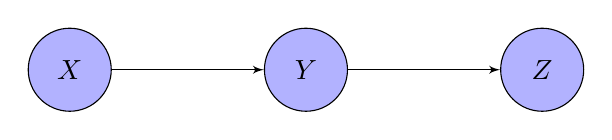
\begin{tikzpicture}[node distance=3cm,auto,>=latex',every node/.append style={align=center}]
    \node [int,  fill = white!70!blue] (a)              {$X$};
    \node [int,  fill = white!70!blue]           (c) [right of=a] {$Y$};
    \node [int,  fill = white!70!blue] (e) [right of=c] {$Z$};
    \path[->, auto=false] (a) edge node {} (c)
                          (c) edge node {} (e) ;

\end{tikzpicture}
\caption{Depiction of a SIR model where $X=S, Y=I,$ and $Z=R$.  One can only get the disease once in this model.}\label{fig::sir}
\end{figure}
An outbreak occurs if the rate of change of infectious individuals is positive, $\frac{dY}{dt} > 0$, or equivalently,
\begin{align*}
  \frac{dY}{dt} &> 0 \\
  \implies \frac{\beta X Y}{N}  - \gamma Y &> 0 ,\\
\implies  Y \left ( \beta \frac{X}{N} - \gamma \right ) & > 0\\
\implies   \frac{\beta}{\gamma} &> \frac{N}{X}.
\end{align*}
That is,  the rate of new infections is greater than the rate of recovery.  So as long as the number of susceptibles is large compared to the total population, $\frac{X}{N} \approx 1$, then an outbreak will occur if $\rr >1$,
\begin{align*}
  \rr \overset{def}{=} \frac{\beta}{\gamma} > 1.
  \end{align*}
  In order to incorporate randomness into the model, we add noise, namely,
  \begin{align}\label{eq:sir-noise}
    X_{obs}(t) &= X(t) + \epsilon_{X,t}\\
    Y_{obs}(t) &=  N - X_{obs}(t) -Y_{obs}(t)  \nonumber\\
    Z_{obs}(t) &= Z(t) - \epsilon_{Z,t}. \nonumber
  \end{align}
We are assuming the observations are generated based on the deterministic ODEs presented in Equation \ref{eq:sir} with the addition of time ($t=0, 1, \dots, T$) and compartment dependent noise $\epsilon_{X,t}$ and $\epsilon_{Z,t}$.  Since, $N$, the total population, is constant, then $Y_{obs}$ is adjusted accordingly.

In summary, when we discuss estimators for $\rr$ for the SIR model, we mean to say we are forming an estimator of $\rr$ from the given set of data in Eq. \ref{eq:sir-noise},
\begin{align*}
  \textnormal{Data} &= \left \{\left (X_{obs}(t), Y_{obs}(t), Z_{obs}(t) \right ) : t=0, 1, \dots, T\right \}, \\
  \hat{\rr} &= m(\textnormal{Data}),
\end{align*}
where $m$ is a function of the data.

Good properties of an estimator may include (1) being a consistent estimator
\begin{align*}
  \hat{\rr} \overset{P}{\to} \rr \textnormal{ as } T\to \infty
\end{align*}
or (2) converging to a known probability distribution,
\begin{align*}
\hat{\rr} \overset{d}{\to} F.  
\end{align*}
As we are interested in the hypothesis
\begin{align*}
  H_0:\;& \rr > 1 \\
  H_A:\;& \rr \le 1
\end{align*}
Then for some $\alpha \in [0,1]$, we would like to know for some $a, b >0$
\begin{align*}
P(a \le \hat{\rr} \le b) = 1 - \alpha,  
\end{align*}
the second property is particularly desirable, as we could find $a$ and $b$ from the distribution $F$.  At any rate, we would like to be able to estimate $a$ and $b$ for a given $\alpha$-level.  We could also make similar hypothesis tests such as that the $\rr$ for H1N1 influenza is greater than the reported $\rr$ for seasonal influenza.

\section{Overview of \wxxsir methods to estimate $\rr$ for the SIR model}
\label{sec:methods} 

In this section, we describe the \wxxsir methods in detail, including advantages and disadvantages of each.

\subsection{Least Squares ($\beta$, $\gamma$) (LS)}\label{least-squares-beta-gamma}
Our first approach to estimate $\rr$ in the SIR model is to minimize the joint mean square error for the data collected at each time point and use the plug-in estimator found in Equation \ref{eq:sirls}.  In particular, we find

\begin{align*}
(\hat{\beta}, \hat{\gamma} )&=\arg \min_{\beta, \gamma} \sum_{t} \left [ \left (X_{obs}(t) - X(t)\right )^2 + \left ( Z_{obs}(t) - Z(t) \right )^2 \right ]
\end{align*}
Then the least squares (LS) estimate for $\rr$ is given by Equation \ref{eq:sirls},
\begin{align}\label{eq:sirls}
  \hat{\rr}= \frac{\hat{\beta}}{\hat{\gamma}}.
\end{align}

This method is sometimes used to estimate $\hat{\beta}$ and $\hat{\gamma}$ via a grid search of $\beta$ and $\gamma$ but can also be done with more sophisticated optimiization algorithms.  Since we cannot explicitly write down the partial derivatives of $S$, $I$, and $R$ with respect to $\beta$ and $\gamma$, we can only use minimization algorithms which do not rely on an explicit gradient such as Nelder-Mead simplex minimization \citep{nelder-mead1965}.

A reasonable question one may ask is why use the $L_2$-norm as opposed to $L_1$ or some other similarity score.  A possible answer is that if we were to assume Gaussian noise, then the $L_2$-norm would be equivalent to the maximum likelihood estimation.  Another answer is that $L_2$ is a continuously differentiable function and hence is easier to compute, which allows for sensitivity analysis to  be conducted more easily.  Finally, LS can be done without writing down explicit assumptions on the noise within the model.  However, we cannot guarantee properties of consistency or convergence to a known distribution without more explicit assumptions.  

On the other hand, least squares is easy to implement in software such as \texttt{R}'s \texttt{optim()} function, and as we see in Section \ref{sec:results} produces comparable methods to other methods.  Least squares and similar variants have been used to estimate $\rr$ in \cite{majumder2016}.

\subsection{Reparametrized Least Squares ($\rr$, $\gamma$) (ReLS)}\label{reparametrized-least-squares-rux5f0-gamma}

In the previous method (Section \ref{least-squares-beta-gamma}), we estimated $\beta$ and $\gamma$ and then estimated $\rr$.  However, it is possible to directly estimate $\rr$ if we reparametrize the ODEs in Equation \eqref{eq:sir} directly with \(\rr\) and \(\gamma\), using the relation $\rr = \frac{\beta}{\gamma}$,

\begin{align*}
  \left \{
  \begin{array}{cl}
    \frac{dX}{dt} &= - \rr \gamma Y \frac{X}{N}\vspace{.5em}\\
    \frac{dY}{dt} &=  \rr \gamma Y \frac{X}{N}  - \gamma Y\vspace{.5em} \\
    \frac{dZ}{dt} &=  - \gamma Y 
  \end{array}
  \right . .
  \end{align*}
We find
\begin{align*}
(\hat{\rr}, \hat{\gamma} ) &= \text{argmin}_{\rr, \gamma} \sum_{t} \left [ \left (X_{obs}(t) - X(t)\right )^2 + \left ( Z_{obs}(t) - Z(t) \right )^2 \right ]
\end{align*}
We use the $\hat{\rr}$ directly from the above estimation problem, which again can be solved with a grid search or another optimization process.  It may be surprising that this method leads to different results than simply using least squares.  One reason we obtain different results may be attributed to better numerical precision as there is one fewer step to obtain an estimate for $\rr$.  However, we also see that this method further results in smaller standard errors than in LS, which we discuss more in Section \ref{sec:results}.

Like LS, while we have no explicit parametric assumptions on the noise, we also are uncertain of any theoretical properties of our resulting estimator.  Likewise, the same difficulties in sensitivity analysis arise as in LS.



\subsection{Linear Model Approximation (LMA)}\label{linear-model-approximation-degree-10}

The SIR ODEs in Eq. \ref{eq:sir} have no known closed form solution, and so we use numerical integration to obtain approximate solutions.  In addition to this, data collected from real diseases are typically very noisy to begin with.  \cite{chang2017} showed that an SIR model may be well approximated by a linear model.  We use this approach here to estimate $\rr$.

Specifically, we estimate two linear polynomials in \(t\) with degree $K$  to \(X_{obs}\)
and \(Z_{obs}\) using least squares to find the coefficients $\{(\hat{x}_k,
\hat{z}_k)\}_{k=1, \dots, K}$,
\begin{align*}
\hat{X}(t) &= \sum_{k=0}^K \hat{x}_k t^k\\
{\hat{Z}}(t) &= \sum_{k=0}^K \hat{z}_k t^k
\end{align*}
Then, we estimate the derivatives as
\begin{align*}
\hat{X}^\prime(t) &= \sum_{k=1}^K k \hat{x}_k t^{k-1}\\
\hat{Z}^\prime(t) &= \sum_{k=0}^K k \hat{z}_k t^{k-1}
\end{align*}
Following,  an estimator for \(\rr\) is derived from the ODEs in Equation \eqref{eq:sir},
\begin{align}
  - \frac{X^\prime}{Z^\prime}&= \rr \frac{X}{N} \nonumber\\
  \rr &=       -\frac{X^\prime}{
        Z^\prime} \cdot \frac{N}{X} \nonumber\\
  \hat{\rr} &= -\frac{\hat{X}^\prime(0)}{ \hat{Z}^\prime(0)} \cdot \frac{N}{\hat{X}(0)}. \nonumber
  \end{align}
  Here, $K$ is arbitrary and should be selected using some criterion such as AIC.  Besides optionally deciding on the degree of polynomials to fit, this model is simple to implement and gives comparable results to using least squares with the SIR model.  The time $t=0$ is used to best capture the initial outbreak.

  An advantage of using this estimation method is that it is simple to implement using any linear modelling software.  On the other hand, we are assuming $X(t) = \hat{X}(t)$ and so if the data truly follows a SIR model, then we will likely have a biased result for $\rr$.  Using this method, we are able to check how sensitive $\rr$ is to the degree of the fitted polynomial.

\subsection{Linear Model Approximation, All Time Points (LMAT)}\label{linear-model-approximation-all-time-points-degree-10}

The above formulation (Section \ref{linear-model-approximation-degree-10}) of a linear model approximation only uses the estimate at time $t=0$ to estimate $\rr$.  We can instead, use all time points $O$ available to estimate $\rr$.  We fit a polynomial in \(t\) with degree \(K\) to \(X_{obs}\)
and \(Z_{obs}\) as above, with a slight modification in how we estimate
\(\rr\),
\begin{align*}
  \hat{\rr} &= \frac{1}{O} \sum_t \frac{-\hat{X}^\prime(t)}{\hat{Z}^\prime(t)} \cdot \frac{N}{X(0)} 
\end{align*}
The intuition is that $\frac{-X^\prime(t)}{Z^\prime(t)}$ is constant in $t$, but due to our approximations with the linear model, this is no longer the case.  Here, we average over the different possible values of $\rr$, estimated at different times.  An advantage to this approach is that we have a more robust estimate of $\rr$ than just using one time point.  Like in LMA, we can examine how sensitive $\rr$ is to the order of the polynomial $K$.


\subsection{Incidence to Prevalence Ratio (IPR)}\label{incidence-to-prevalence-ratio}
The incidence to prevalence ratio (IPR), described by \cite{Nishiura2009}, is another intuitive method to calculate $\rr$ as it incorporates some of the most basic epidemiological quantities, incidence and prevalence.

In terms of data from the SIR model, incidence $J(t) \approx -(X(t+1) - X(t))$, and the IPR$(t) = \frac{J(t)}{Y(t)}$.  This method assumes that we have some prior knowledge about $\gamma$, the recovery rate.  Thus we use as our estimate,
\begin{align*}
\hat{\rr} &= \textnormal{IPR}(t) \cdot \frac{1}{\gamma}
\end{align*}

Here we assume that the time step is small enough to approximate the incidence.  The advantage of this method is that incidence data is generally readily available as is prevalence data for certain diseases such as HIV.  However, as one is required to have prior knowledge about $\gamma$, it may be easier to directly estimate $\rr$ with one of the many other methods described that does not require a prior knowledge about $\gamma$.  Again, we are using only one time point to estimate $\rr$.  This model is agnostic to assumptions on the noise, but again, it is unclear if this is an unbiased or consistent estimator of $\rr$.

\subsection{Smoothed Incidence to Prevalence Ratio (SIPR)}
We use the same method as above, IPR, but first estimate splines with $K$ degrees of freedom, where $K$ is small, $\hat{X}(t)$ and $\hat{Y}(t)$, to fit to $X_{obs}$ and $Y_{obs}$, respectively.  Then  $J(t) \approx -(\hat{X}(t+1) - \hat{X}(t))$, and the $\hat{\textnormal{IPR}}(t) = \frac{J(t)}{\hat{Y}(t)}$.  Then
\begin{align*}
\rr &= \hat{\textnormal{IPR}}(t) \cdot D
\end{align*}
The advantage of this method is that it creates a less variable estimate than estimating IPR using only one point.  It has the same disadvantages as the regular IPR ratio in that it requires knowledge about $\gamma$.

%%%%%%%%%%%%%%%%%%%%%
\subsection{Log-Linear (LL)}
\cite{harko2014exact} were able to reduce the SIR model to one ODE.  From this, we can derive the following,
\begin{align}
  X(t) &=  X(0) e^{\frac{-\beta}{\gamma}\frac{Z(t)}{N}} \nonumber\\
  \log \frac{X(t)}{X(0)} &=  \frac{-\beta }{\gamma}\frac{Z(t)}{N} \nonumber\\
  \log \frac{X(t)}{X(0)} &=  -\rr \frac{Z(t)}{N}. \label{eq:harko_lin}
\end{align}

Thus, we can regress the left hand side in Eq. \ref{eq:harko_lin} on $Z(t)$, the number of recovered individuals, with $\rr$ as the coefficient of $Z(t)/N$ and with an intercept term of $\beta_0=0$ to obtain an estimate of $\rr$,
\begin{align*}
  \hat{\rr} = -\frac{\sum_{t=0}^T \log \frac{ X(t)}{X(0)}}{\sum_{t=0}^T\frac{Z(t)}{N}}.
\end{align*}
This method says that for a one percent increase in number of recovered individuals, we expect the ratio of number of previous susceptibles to number of new susceptibles to increase by $e^{\rr}$,
\begin{align*}
  \log \left ( X(t+1)/ X(0) \right ) - \log \left ( X(t)/X(0) \right ) &= - .01\rr\\
  \log \left ( X(t+1) \right ) - \log \left ( X(t) \right )  &=- .01\rr\\
  \log \left ( X(t) / X(t+1) \right ) &= .01\rr\\
  \frac{X(t)}{X(t+1)}  &\approx e^{\rr}.
\end{align*}

The advantages of this method are many.  One, the estimate of $\rr$ is highly interpretable.  Two, an assumption of Gaussian noise in Equation \ref{eq:harko_lin} is not as egregious as in the other methods to estimate $\rr$ because we are looking at a log transformation of the the percent of suceptibles instead of raw variables.  As a consequence, we may be able to make a case where we the resulting estimate of $\rr$ is unbiased and a consistent estimator.  Finally,  this method is easily implemented using any linear modelling software.  

\subsection{Markov chain estimation (MC)}
A natural approach to epidemic modelling is that of Markov chains (MC), since it is assumed an individual's next state is only dependent on its current state and the current states of other individuals.  Much work has been done over the years in this specific field including asymptotic behavior, continuous time MC, confidence intervals, and more \citep{jacquez1991,gani1995,daley2001epidemic}.  We present one simple instantiation of the model, the discrete time case, which traces its origin back to the Reed-Frost model \citep{abbey1952}.

In this method, the number of susceptibles at the next step, $X(t+1)$, has a Binomial distribution based on the contacts with the current number of infectious, $Y(t)$ and the current number of susceptibles.  That is $X(t+1) \sim \text{Binomial}\left(X(t), \alpha^{Y(t)}\right)$, where $\alpha$ is the probability of avoiding infection from an infective.  One can write out the likelihood for $\alpha$ in this model, namely,
\begin{align*}
\mathcal{L}\left ( \alpha ; \textnormal{data}\right ) \propto \prod_{t=0}^{T-1}\left ( \alpha^{Y(t)} \right )^{X(t+1)} \left (1- \alpha^{Y(t)} \right )^{X(t) - X(t+1)}.
\end{align*}
Maximizing the likelihood yields an estimate for $\alpha$,
\begin{align*}
\hat{\alpha} = \arg \max_{\alpha} \mathcal{L}\left(\alpha; \textnormal{data} \right ).
  \end{align*}
 \cite{barbour2004} report that the estimated reproduction number is thus,
\begin{align}\label{eq:r0-mc}
\hat{\rr} &= \log \left ( \frac{1}{1-\hat{\alpha}}\right ).
\end{align}

This method typically allows for more than just the reproduction number to be estimated.  Through recursion, one can calculate the probability of having a given number of susceptibles and infected at each time step, and hence the entire probability distribution may be known.

The advantages of this model are its simplicity of interpretation and ability to generate a whole probability distrubtion for $(X(t), Y(t))$.  We have explicitly stated how randomness enters the model so it is up to the researcher to check whether this assumption is a good fit.  Also, it is possible to simulate how sensitive $\hat{\rr}$ is to $\hat{\alpha}$.





\subsection{Sequential Bayes (SB)}\label{sec:seqbayes}

Described by \cite{bettencourt2008} and summarized in \cite{obadia2012r0}, the sequential Bayes method is a Bayesian approach to an approximation of the classic SIR model.  The approximated SIR model assumes that the incidence at $t+1$, $J(t+1)$ has a Poisson distribution, with $\gamma$ as the  average inverse of the infectious period. In order to estimate $\rr$, we must have some idea about $\gamma$,
\begin{align*}
J(t+1)  \sim \textnormal{Poisson}( J(t) \exp \left \{  \gamma (\rr-1)\right \})
\end{align*}
Then, the posterior distribution of $\rr$ given the previous days' incidence is
\begin{align*}
  P(\rr | J_0, \dots, J_{t+1}) = \frac{P(J_{t+1} | \rr, J_0, \dots, J_t)P(\rr| J_0, \dots, J_t)}{P(J_0, \dots, J_{t+1})}.
\end{align*}
This method is sequential in that the prior distribution for $\rr$ comes from the previous day.  The initial prior for $\rr$ is assumed to be flat.  This method results in a posterior distribution from which credible intervals may be obtained.  This method assumes, initial growth in incidence to be exponential, and homogeneous mixing of populations as with any compartment model.  The advantages of this method are that of the ability to obtain an entire posterior distribution, whereas many other methods are difficult to even find an estimate of the variance.  Disadvantages include strict assumptions about the distributions and computational time required to estimate the relevant parameters.

\subsection{Exponential Growth (EG)}\label{sec:expgrowth}
%% nishiura, majumder, IDEA model -- sum of squares (santillana2016)
%% An IDEA for short term outbreak projection: nearcasting using the basic reproduction number.  (fisman2013, fisman2014)
%% chowell 2008 - parametric bootstrap for a model they made up, but sort of empirical.
Many researchers employ an assumption of exponential growth of the number infectious through times $t=0, 1, \dots, T^* <T$ \citep{wallinga2007generation,fisman2014,nishiura2016,majumder2016,towers2016}.
\cite{wallinga2007generation} report that the effective reproduction number $\mathcal{R}_t$ and hence the initial reproduction number $\rr$ may derived using the fact that infection ``counts increase exponentially in the initial phase of an epidemic.''  We then have to estimate $r$, the \textit{per capita} change in the number of new cases per unit of time and $\omega$ the serial interval, the distribution of time between a primary and secondary infection. Then, we have
\begin{align}\label{eq:lotka}
\rr = \exp{(r \omega)}.
\end{align}
Equation \eqref{eq:lotka} is derived from a demographic view using the Lotka-Euler survival equations which come from the fields of demography, ecology, and evolutionary biology.

\cite{wallinga2007generation}, instead, use a moment generating function expression for $\rr$.  With $\omega(t)$ as the serial interval, then
\begin{align*}
\rr^{-1} &= \frac{1}{M(-r)} = \int_{a=0}^\infty e^{-rt}\omega(t)dt.
\end{align*}
\cite{wallinga2007generation} specifically derive an estimate for $\rr$ for the SIR model.  They assume that the rate of leaving the infectious stsate, $\gamma$ is constant as is the rate of making contacts during the infectious stage.  Then, the duration of a serial interval is an exponential distribution with mean $\gamma^{-1}$, the moment generating function is then,
\begin{align*}
  M(-r) = \frac{\gamma}{\gamma + r},
\end{align*}
and the resulting estimate of $\rr$ is
\begin{align}\label{eq:r0-eg}
  \hat{\rr} = 1 + \frac{\hat{r}}{\hat{\gamma}},
\end{align}
where $\hat{r}$ and $\hat{\gamma}$ are estimates of the $r$ and $\gamma$, respectively.  The parameter $\hat{\gamma}$ is often assumed to be fixed or tried with a sequence of serial intervals \citep{majumder2016}.  We may estimate $\hat{r}$ using ordinary linear regression, namely,
\begin{align*}
  \log \left  (\frac{Y(t)}{Y(0)} \right )&= rt + \epsilon_t\\
  \epsilon_t &\sim N(0, \sigma^2),
\end{align*}
which results in
\begin{align}\label{eq:exp-growth}
  \hat{r} &= \frac{\sum_{t=0}^{T^*}\left  (\frac{Y(t)}{Y(0)} \right )}{\sum_{t=0}^{T^*}t}.
\end{align}



For the above estimate of $\rr$, we observe the duration of serial intervals in a period of exponential growth of the number of infectious individuals.  Deciding when exponential growth occurs and which data points to use to estimate $\rr$ may be difficult.  We can use sensitivity analysis to see how the estimate $\rr$ changes as we increase or decrease $T^{*}$, the number of time points used. The reader may notice some similarities to the estimate for $\rr$ in Equation \eqref{eq:r0-eg} and from the log-linear model in Equation \eqref{eq:harko_lin}.  This method is a simplification of the SIR model as the $R$ compartment is not used to estimate $r$, only the recovery rate $\gamma$. 

An advantage to this method are its (and similar adaptations) prevalence in the literature, which allows one to to compare estimates $\rr$ directly to one another.  Another advantage is its flexibility.  Here, we assumed the serial interval has an exponential distribution, but this is not a requirement and other distributions may be used (see \cite{wallinga2007generation}).  However, a disadvantage to this method is that is a simplification of the SIR model and we have to decide how many time points to use to estimate the exponential growth rate of infectious.  Another disadvantage to this method is that one also has to decide how to treat the additional paramter $\gamma$, whether to treat it as fixed, a range of fixed values, or even having a probability distribution.


\subsection{Incidence Decay and Exponential Adjustment (IDEA)}\label{sec:idea}
The Incidence Decay and Exponential Adjustment (IDEA) model is a way to account for a declining effective reproduction number of time due to both depletion of susceptible individuals and spontaneous and planned control activities and behaviors'' \citep{fisman2013}.  They model the incidence counts during the $t$th interval, $J(t),$ as
\begin{align*}
  J(t) &= \left [ \frac{\rr}{(1 + d)^t}\right ]^t,
\end{align*}
where $d$ is a dampening or discount factor.  As $d$ increases, the incidence at time $t$  decreases. The estimate for $\rr$ is obtained by minimizing the sum of squares over $\rr$ and $d$,
\begin{align*}
  \hat{\rr} &=  \arg \min_{\rr,d} \sum_{t=0}^{T^*}\left (J_{obs}(t) - J(t) \right)^2.
\end{align*}
The method presented in \cite{fisman2013} is a mathematical, rather than statistical model.  Sensitivity analysis is conducted with respect to $T^*$, $d$, and $\rr$, and lower and upper bounds are reported as a result of this analysis.

Advantages of this method include its usefulness in estimating $\rr$ \citep{fisman2014,majumder2016}.  Additionally, this model may be employed to address the effect of control measures and better estimate the final size of an epidemic.  A disadvantage to this model is that its upper and lower bounds do not correspond to CIs.  Also, in this method we must select the interval size of the incidence counts.

\section{Confidence and Credible Intervals}
\label{sec:ci}

Estimating $\rr$ is difficult and estimating $V[\rr]$, the variance and confidence or credible intervals (CI) is even more so.  We describe general methods which may be applicable to estimate the variance.  In particular, we describe three methods 1) the delta method, 2) the block bootstrap, and 3) posterior distributions.




\subsection{Delta Method}\label{delta-method}

When the method estimates \(\beta\) and \(\gamma\) instead of \(\rr\) directly, we use the delta method approximation to calculate the
variance of \(\rr\). Here, we know \(\rr = h(\beta, \gamma) = \frac{\beta}{\gamma}\). Then \(\bigtriangleup h = (\frac{1}{\gamma},  -\frac{\beta}{\gamma^2})^T\) and \(V[\rr] = \bigtriangleup h^T \Sigma_{\beta, \gamma} \bigtriangleup h\), where \(\Sigma_{\beta, \gamma}\) is covariance matrix of \(\beta\) and \(\gamma\).

This estimate assumes that the distribution of $\beta$ and $\gamma$ are asymptotically normal.  Here, we use the relationship of $\rr = \frac{\beta}{\gamma}$ in order to estimate the variance, which is specific to the SIR model.  This method may be extended to other frameworks such as the SEIR model.  The advantages of the delta method are that since the Next Generation Matrix \citep{diekmann2009} posits a recipe to derive $\rr$, then it is theoretically possible to use the delta method to derive an expression for the variance of $\rr$ for any compartment model.

\subsection{Block Bootstrap}

The block bootstrap is a variant of the bootstrap in which the $n$ observations are dependent on one another.  In contrast to the original bootstrap, the block bootstrap partitions consectutive observations into $k$ blocks with block-length $b$ ($n=kb$).  These are non-overlapping partitions or blocks, although there are variants for which blocks can overlap.  For iteration $\ell$, one samples $k$ blocks uniformly with replacement and estimates $\hat{\rr}_b$, repeating the sampling and estimation for a total of $L$ estimates of $\hat{\rr}$.  Then
\begin{align*}
  V\left [ \hat{\rr} \right ] &\approx V\left [\hat{\rr}_\ell \right ].
\end{align*}
More about the asympotic distributions of the blockwise-bootstrap can be found in \cite{cao1999}, along with descriptions of variants of the block bootstrap.

The asympotic properties hold when the stochastic process is $m$-dependent, that is when observations $t, t+1, \dots$ and $s, s+1, \dots$ are independent whenever $s+m < t$ and under some smoothness conditions of the statistic used to estimate $\rr$.

A choice one must make in the block bootstrap is the block size $b$.  One simple recommendation is to take $b= n^{1/3}$, which is derived from the asymptotic mean square error of the method.


\subsection{Posterior Distribution}
Here, we assume $\rr$ is a random variable and the data is fixed.  Following the notation of \cite{wasserman2004}, then the posterior distribution $f(\rr | \textnormal{data})$ is is proportional to the likelihood of observing the data given $\rr$, $\mathcal{L}(\textnormal{data}|\rr)$, multiplied by our prior on $\rr$, $f(\rr)$. 
\begin{align*}
f(\rr | \textnormal{data} ) \propto \mathcal{L}(\textnormal{data} | \rr) f(\rr)
\end{align*}
 Typically, the posterior is either estimated using conjugate distributions for the likelihood and prior or through Markov Chain Monte Carlo (MCMC) to simulate a posterior distribution $\hat{F}$ such that
\begin{align*}
\hat{F} \overset{d}{\to} f(\rr| \textnormal{data}).
\end{align*}
Then commonly, $\hat{\rr} = \hat{F}_{.5}$, the median of $\hat{F}$.  Correspondingly, the 95\% credible interval is $\left[\hat{F}_{.05}, \hat{F}_{.95} \right ]$. Advantages of this method include having an entire distribution compared to a point estimate.  A disadvantage is that using conjugate priors may not be justified for the given data and MCMC may be computationally intractable.  One should note that these 95\% credible intervalss are not the same as confidence intervals as the ``true'' value of $\rr$ may not be contained in the credible intervals 95\% of the time.




%%%%%%%%%%%%%%%

\section{Methods}\label{sec:sim-res}

We compare the performance of the SIR models on simulated data from both the SIR as well as other models. In all of these simulations, we first generate data from the models under known conditions, then we add on errors drawn from known distributions variances to each time point,
\begin{align}\label{eq:sim-models}
  X_{model}(t) &= f(t) + \epsilon_{X,t} \\
  Y_{model}(t) &= g(t) + \epsilon_{Y,t} \nonumber\\
  Z_{model}(t) &= N - X(t) - Y(t)\nonumber 
\end{align}
We adjust the recovered compartment $Z$ so the total population is constant. 
We simulate with two different types of error distributions, Gaussian and autoregressive,

\noindent \textbf{Gaussian (Norm) ($X_{G}$, $Y_{G}$, $Z_{G}$)}
\begin{align*}
  f(t) &= X(t) \\
  g(t) &= Y(t) \\
  \epsilon_{X,t} &\sim N(0, \sigma_X^2) \\
  \epsilon_{Y,t} &\sim N(0, \sigma_Y^2)
\end{align*}
\textbf{Autoregressive (AR) ($X_{AR}$, $Y_{AR}$, $Z_{AR}$)}
\begin{align*}
  f(t) &= \rho X_{obs}(t-1) \\
  g(t) &= \rho Y_{obs}(t-1) \\
  \epsilon_{X,t} &\sim N(0, \sigma_X^2) \\
  \epsilon_{Y,t} &\sim N(0, \sigma_Y^2).\\
\end{align*}
For both the Gaussian and AR dataset, we form an additional dataset which enforces the monotonicity of X and Z via the Pool Adjacent Violators Algorithm (PAVA), described by \cite{friedman1984}).  Here, we adjust $Y$ so the constant population is maintained.

\noindent \textbf{Gaussian-PAVA (Norm-M) ($X_{GP}$, $Y_{GP}$, $Z_{GP}$)}
\begin{align*}
 X_{GP}(t) &= \textnormal{PAVA}(X_G(t)) \\
  Y_{GP}(t) &= N - X_{GP}(t) - Z_{GP}(t) \\
  Z_{GP}(t) &= \textnormal{PAVA}(Z_G(t)) \\
\end{align*}
\textbf{Autoregressive-PAVA (AR-M) ($X_{ARP}$, $Y_{ARP}$, $Z_{ARP}$)}
\begin{align*}
  X_{ARP}(t) &= \textnormal{PAVA}(X_{AR}(t)) \\
  Y_{ARP}(t) &= N - X_{ARP}(t) - Z_{ARP}(t) \\
  Z_{ARP}(t) &= \textnormal{PAVA}(Z_{AR}(t)) 
\end{align*}
This gives us a total of four error structures for each set of conditions: Gaussian (Norm), Gaussian monotone (Norm-M), autoregressive (AR), and autoregressive monotone (AR-M) for a given set of parameters $(\beta, \gamma, O, X(0), Y(0), Z(0), \sigma_X, \sigma_Y, N)$, the infection rate; recovery rate; total number of time points; initial conditions for number of susceptibles, infectious, and recovered individuals, the standard deviation for both the susceptible and infectious compartments, and the total population, respectively.

\subsection{SIR Data}

We first simulate a ``baseline'' data set from the SIR model under the following conditions: 

\textbf{Baseline Dataset}
\begin{center}
	
	$\beta$ = 0.06, $\gamma$ = 0.03 ($\rr$ = 2)
	
	Number of time steps $O$: 365
	
	Starting X size ($X(0)$): 99950
	
	Starting Y size ($Y(0)$): 50
	
	Starting Z size ($Z(0)$): 0 
	
	$\sigma_X$: 100
	
	$\sigma_Y$: 5
	
	Total population $N$: 100000

        Error: Gaussian.
	
      \end{center}

This baseline data set      

% We then generate different SIR data sets, changing the one of the conditions for simulation each time and using the baseline SIR data as our basis for comparison. The different data sets generated are shown in the following table:

% \begin{table}[h]
% 	\centering
% 	\resizebox{\textwidth}{!}{
% 		\begin{tabular}{@{}lll@{}}
% 			\toprule
%                   \textbf{Parameter Values ($\beta, \gamma$)}        & \textbf{Starting Compartment Sizes ($X_0, Y_0$)}            & \textbf{Variance of Added Errors ($\sigma_X, \sigma_Y$ )}       \\ \midrule
%                   (0.06, 0.001)            & (99000, 1000)                           & (50, 2)                     \\
%                   (0.06, 0.04)             & (99900, 100)               & (500, 20)     \\
%                   (0.06,.03) & (99950, 50) & (100, 5)\\
%                   (0.06, 0.06)             & (99990, 10)             & (2500, 100)           \\
%                   (0.06, 0.24) & (99999, 1) & (10000, 500)                                      \\ \bottomrule
% 		\end{tabular}
% 	}
% 	\caption{Table of data sets.}
% 	\label{tab:datasets}
% \end{table}

\subsection{Other Models}

To test how well the SIR models perform under misspecification, we simulate data from other models. While we will not have a ``known'' $\rr$ value to compare our results to, this will allow us to see if the models give us reasonable results when the data do not come from the SIR model. We simulate data from polynomials of degree 1 and 4 with respect to the time step, using a monotonically increasing function for the $X$ compartment and a monotonically decreasing function for the $Z$ compartment. The sum of these is subtracted from the constant total population to get the $Y$ compartment. We also generated data from a linearized version of the three compartment SIR model with the following ODEs:

\begin{eqnarray*}
	\frac{dX}{dt} &=& -\beta Y \\
	\frac{dY}{dt} &=& \beta Y - \gamma Y \\
	\frac{dZ}{dt} &=& \gamma Y.
\end{eqnarray*}

The data from the linear SIR model were simulated under the following conditions:

\begin{center}
	
	$\beta$ = 0.06, $\gamma$ = 0.05; $\rr$ = 1.2
	
	Number of time steps: 365
	
	Starting X size ($X_0$): 99950
	
	Starting Y size ($Y_0$): 50
	
	Starting Z size: 0 
	
	$\sigma_X$: 10
	
	$\sigma_Y$: 1
	
	Total population: 100000.
	
\end{center}

\section{Results}\label{sec:results}
There are numerous aspects to consider when using a method to estimate $\rr$.  Among these include values of both the infection and recovery rate $(\beta, \gamma)$, the number of data points available (time $T$), the total size of the population ($N$), the initial percent of susceptible individuals $\left (\frac{X(0)}{N}\right)$, the initial percent of infectious individuals $\left (\frac{Y(0)}{N}\right )$, and  the magnitude of the variance of both the number of susceptibles and the number of infectious ($\sigma_X, \sigma_Y$).  We first examine our baseline data, and then we examine each of these aspects individually.

\subsection{Baseline}\label{sec:res-base}

\begin{figure}
  \centering
  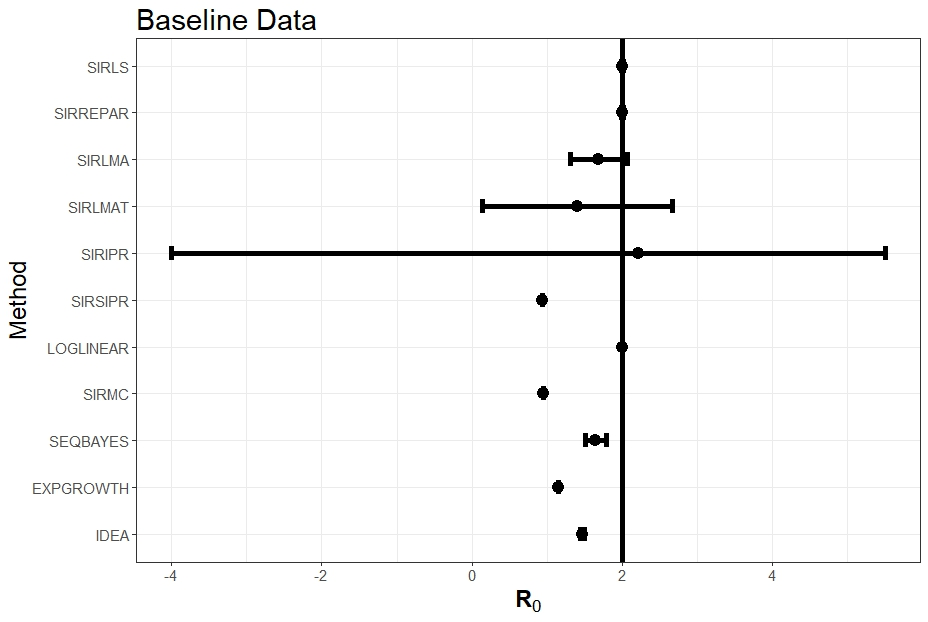
\includegraphics[scale=0.5]{images/BaseBase.jpeg}
  \caption{Forest plots of estimates of $\rr$ for the \xxsir methods for the baseline data set $(\beta=.06, \gamma=.03, O=365, X(0)=99950, Y(0)=50, Z(0)=0, \sigma_X=100, \sigma_Y=5, N=10^5)$.  The points are the estimates of $\rr$ and the lines denote $\pm 2\cdot $Std. Err.  The red line is the true $\rr$ value.}
  \end{figure}

\begin{table}[H]	
	\centering
	\begin{tabular}[t]{l|r|r}
		\hline
		Model & Estimate & Std. Err\\
		\hline
		SIRLS & 1.9999711 & 0.0055923\\
		\hline
		SIRREPAR & 1.9997340 & 0.0049939\\
		\hline
		SIRLMA & 1.6863640 & 0.1886132\\
		\hline
		SIRLMAT & 1.4063227 & 0.6309170\\
		\hline
		SIRIPR & 4.4203632 & 12.3593415\\
		\hline
		SIRSIPR & 1.8870824 & $<$ 1e-07 \\
		\hline
		LOGLINEAR & 1.9998072 & 0.0002198\\
		\hline
		SIRMC & 0.9485555 &  $<$ 1e-07 \\
		\hline
		SEQBAYES & 1.6495023 & 0.0672249\\
		\hline
	\end{tabular}
        \caption{Baseline Data $(\beta=.06, \gamma=.03, O=365, X(0)=99950, Y(0)=50, Z(0)=0, \sigma_X=100, \sigma_Y=5, N=10^5)$, $\rr$ Estimates and Standard Errors}\label{tab:baseline}
\end{table}

Overall, we see a wide variation in the estimates of and the standard errors for $/rr$ depending on the method used. The methods that rely upon least squares optimization and the log-linear model are the closest to the true $\rr$ value, and they also have fairly small standard error estimates. On the other hand, a lot of the methods appear to underestimate the true $/rr$, and many of them have larger standard errors as well. Some notable exceptions include the IPR model, which tends to overestimate $/rr$, and the Markov chain and SIPR models, which appear to have unreasonably small standard errors.

\subsection{Autoregressive Errors}\label{sec:res-AR}

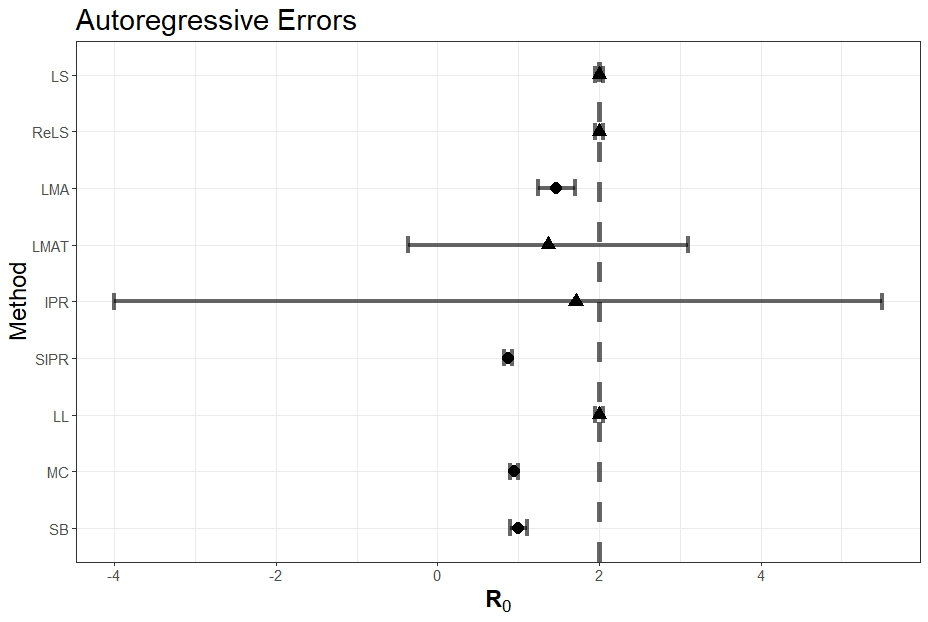
\includegraphics[scale=0.5]{images/AR.jpeg}
\begin{table}[H]
	
	\caption{\label{tab:}Autoregressive Errors, $\rr$ Estimates and Standard Errors}
	\centering
	\begin{tabular}[t]{l|r|r}
		\hline
		Model & Estimate & Std. Err\\
		\hline
		SIRLS & 2.0000198 & 0.0078308\\
		\hline
		SIRREPAR & 1.9998852 & 0.0069901 \\
		\hline
		SIRLMA & 35.656866 & 4815.2163162\\
		\hline
		SIRLMAT & 1.049360 & 4.8830065 \\
		\hline
		SIRIPR & 2.183371 & 7.397726 \\
		\hline
		SIRSIPR & 0.8386350 & $<$ 1e-07 \\
		\hline
		LOGLINEAR & 1.9998203 & 0.0003227\\
		\hline
		SIRMC & 0.9485555 & $<$ 1e-07 \\
		\hline
		SEQBAYES & 1.0000000 & 0.0523424\\
		\hline
	\end{tabular}
\end{table}

With an autoregressive error structure in the simulated data, the log-linear and least squares estimation methods appear to have a similar accuracy. On the other hand, the other models mostly appear to be somewhat less accurate. In particular, the linear regression based models do much worse than in the Gaussian error case. For all of these models, the standard error is larger, which would expect given that the data have a large positive autocorrelation coefficient.


\subsection{Infection and Recovery Rate ($\beta, \gamma$)}\label{sec:res-beta-gamma}

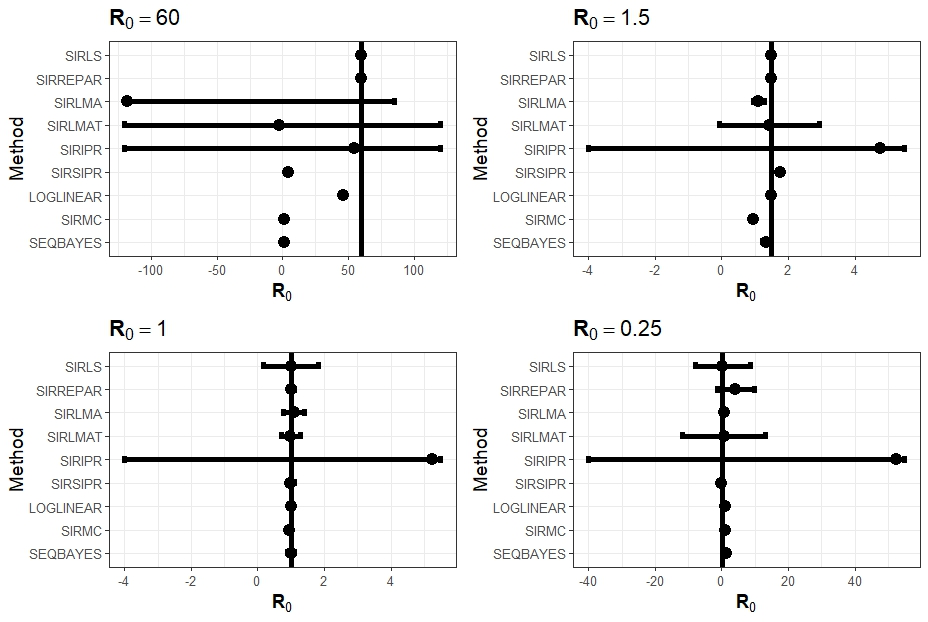
\includegraphics[scale=0.5]{images/parchange.jpeg}

\begin{table}[H]
	
	\caption{\label{tab:}$\gamma = 0.001$, $\rr$ Estimates and Standard Errors}
	\centering
	\begin{tabular}[t]{l|r|r}
		\hline
		Model & Estimate & Std. Err\\
		\hline
		SIRLS & 59.9764682 & 0.0434705\\
		\hline
		SIRREPAR & 59.9951876 & 0.4343984\\
		\hline
		SIRLMA &  -117.9694856 & 101.1885824\\
		\hline
		SIRLMAT & -2.8535930 & 193.6526107 \\
		\hline
		SIRIPR & 54.146506 & 200.2595\\
		\hline
		SIRSIPR & 3.9645187 & $<$ 1e-07\\
		\hline
		LOGLINEAR & 46.3209596 & 0.7797216\\
		\hline
		SIRMC & 0.9485554 & 0.0000001\\
		\hline
		SEQBAYES & 0.9769731 & 0.0517362\\
		\hline
	\end{tabular}
\end{table}

Looking at the case where $\gamma = 0.001$, it appears that most of the models do not handle a very large $/rr$ well. Only the least squares and reparameterized least squares models give very close answers; the IPR and log-linear models give fairly close answers as well. However, the other models do very poorly; they ted to greatly underestimate $/rr$. The linear model approximation does particularly poorly, likely because the linear model does not fit the data well. Several of the models also return extremely large standard errors, meaning they are not very reliable in these cases.

\begin{table}[H]
	
	\caption{\label{tab:}$\gamma = 0.24$, $\rr$ Estimates and Standard Errors}
	\centering
	\begin{tabular}[t]{l|r|r}
		\hline
		Model & Estimate & Std. Err\\
		\hline
		SIRLS & 0.2363274 & 4.1042813\\
		\hline
		SIRREPAR & 4.1795252 & 2.7455569\\
		\hline
		SIRLMA &  0.7074613 & 0.2028765 \\
		\hline
		SIRLMAT & 0.6746914 & 6.2471252 \\
		\hline
		SIRIPR & 181.015802 & 742.1088 \\
		\hline
		SIRSIPR & -0.2484284 & 0.1159769 \\
		\hline
		LOGLINEAR & 0.9912397 & 0.0030505\\
		\hline
		SIRMC & 0.9485811 & 0.0000150\\
		\hline
		SEQBAYES & 1.2354952 & 0.0581801\\
		\hline
	\end{tabular}
\end{table}

The above table corresponds to the case where $\gamma = 0.24$. It appears that a lot of estimation methods do not handle very small $/rr$ well either. None of them are extremely close to truth, except for regular least squares, as most of the tend to overestimate the truth. The IPR is particularly bad in this case. Also, in general, the standard errors are several orders of magnitude larger than in the baseline data.


\subsection{Number of Time Steps ($T$)}\label{sec:res-time}

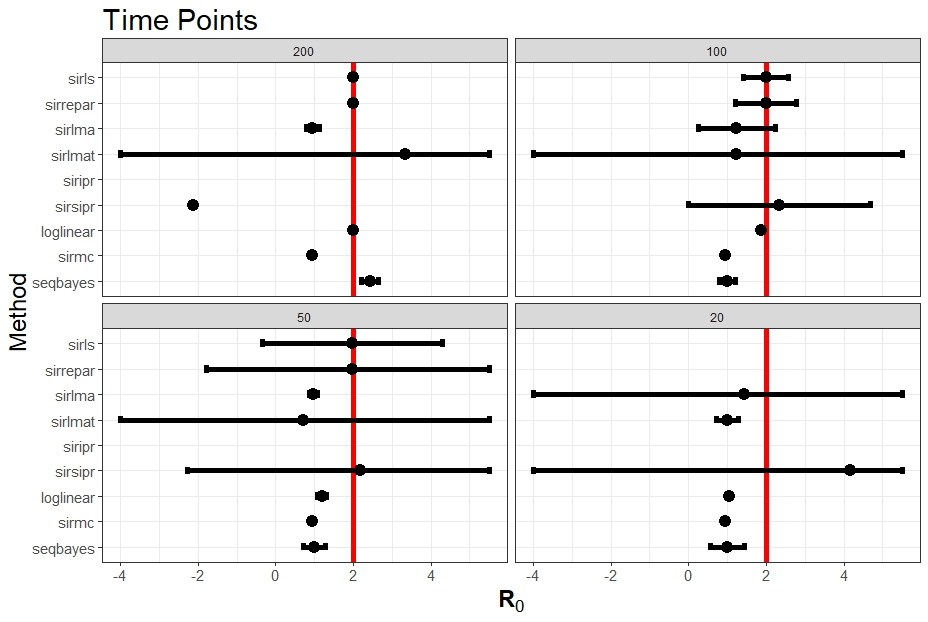
\includegraphics[scale=0.5]{images/time.jpeg}

\begin{table}[H]
	
	\caption{\label{tab:} $T$ = 100, $\rr$ Estimates and Standard Errors}
	\centering
	\begin{tabular}[t]{l|r|r}
		\hline
		Model & Estimate & Std. Err\\
		\hline
		SIRLS & 1.9993392 & 0.0286060\\
		\hline
		SIRREPAR & 1.9994284 & 0.0312814\\
		\hline
		SIRLMA & 0.9496498 & 0.0825419\\
		\hline
		SIRLMAT & 3.3442696 & 21.4895422\\
		\hline
		SIRIPR & 7.3458131 & 16.1288906\\
		\hline
		SIRSIPR & -2.1198897 & $<$ 1e-07\\
		\hline
		LOGLINEAR & 2.0014146 & 0.0017620\\
		\hline
		SIRMC & 0.9485555 & 0.0000001\\
		\hline
		SEQBAYES & 2.4289382 & 0.1102030\\
		\hline
	\end{tabular}
\end{table}

The table above shows the methods applied to the first 100 time steps, out of 365, of a baseline data set. The estimates and standard errors are worse, which we would expect given less data. The results are still relatively close to the full baseline data. There also appears to be less tendency to underestimate $/rr$ compared to a longer time scale.

\begin{table}[H]
	
	\caption{\label{tab:} $T$ = 20, $\rr$ Estimates and Standard Errors}
	\centering
	\begin{tabular}[t]{l|r|r}
		\hline
		Model & Estimate & Std. Err\\
		\hline
		SIRLS & 38.6895520 & 106.2705193\\
		\hline
		SIRREPAR & 22.9645867 & 6.9816713\\
		\hline
		SIRLMA & 1.4418031 & 7.3163878\\
		\hline
		SIRLMAT & 1.0078807 & 0.1424793\\
		\hline
		SIRIPR & 25.7313065 & 35.2926077\\
		\hline
		SIRSIPR & 4.1772451 & 7.3202970\\
		\hline
		LOGLINEAR & 1.0429764 & 0.0276261\\
		\hline
		SIRMC & 0.9485556 & 0.0000005\\
		\hline
		SEQBAYES & 1.0000000 & 0.2236068\\
		\hline
	\end{tabular}
\end{table}

The table above shows the methods applied to the first 20 time steps of a baseline data set. As might be expected, the $/rr$ estimates are wildly inaccurate, and none are very close. The least squares methods are particularly worse in this situation compared to the other data sets. The standard errors are much larger than the baseline, which is to be expected as well due to the small number of data points. This shows that it is extremely difficult to create accurate online estimates of $/rr$ or to estimate $/rr$ without adequate data. 

\subsection{Initial Percentage of Infectious $\left (\frac{Y(0)}{N}\right)$}\label{sec:res-inf}

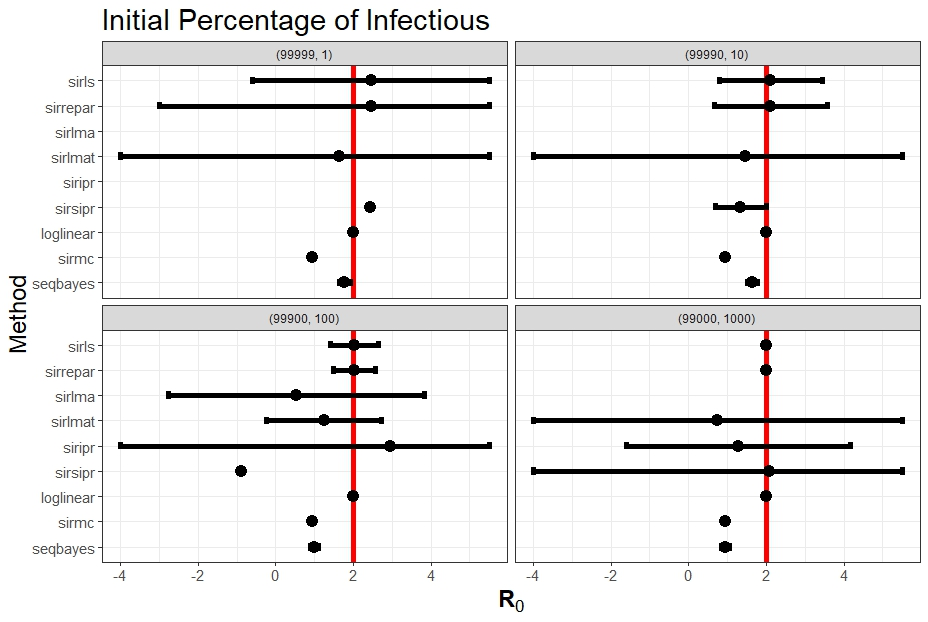
\includegraphics[scale=0.5]{images/start.jpeg}

\begin{table}[H]
	
	\caption{\label{tab:}$Y(0) = 1000$, $\rr$ Estimates and Standard Errors}
	\centering
	\begin{tabular}[t]{l|r|r}
		\hline
		Model & Estimate & Std. Err\\
		\hline
		SIRLS & 1.9995884 & 0.0049609\\
		\hline
		SIRREPAR & 1.9997123 & 0.0034303\\
		\hline
		SIRLMA & -87.5945650 & 66413.128046\\
		\hline
		SIRLMAT & 0.7306100 & 4.681042\\
		\hline
		SIRIPR & 1.285071 & 1.440980\\
		\hline
		SIRSIPR & 1.2522106 & 57.9229822 \\
		\hline
		LOGLINEAR & 1.9995148 & 0.0002828\\
		\hline
		SIRMC & 0.9485555 & $<$ 1e-07\\
		\hline
		SEQBAYES & 0.9728534 & 0.0516270\\
		\hline
	\end{tabular}
\end{table}

The table above shows the methods applied to data where $Y(0) = 1000$, essentially starting at the middle of an epidemic. This data has very large underestimation of $/rr$. The LMA method once again gives a very far estimate, potentially indicating that a linear approximation does not apply in this case. The sample standard errors in this case are actually relatively close to the baseline, and even smaller for some of the methods.

\begin{table}[H]
	
	\caption{\label{tab:}$Y(0) = 1$, $\rr$ Estimates and Standard Errors}
	\centering
	\begin{tabular}[t]{l|r|r}
		\hline
		Model & Estimate & Std. Err\\
		\hline
		SIRLS & 2.468304 & 1.5370731\\
		\hline
		SIRREPAR & 2.469189 & 2.7293667\\
		\hline
		SIRLMA & 10.9282204 & 19.297359 \\
		\hline
		SIRLMAT & 1.624645 & 5.0359845\\
		\hline
		SIRIPR & 774.274659 & 7491.005080 \\
		\hline
		SIRSIPR & 2.4390757 & $<$ 1e-07 \\
		\hline
		LOGLINEAR & 1.999690 & 0.0007731\\
		\hline
		SIRMC & 0.948603 & 0.0000156\\
		\hline
		SEQBAYES & 1.471481 & 0.0634937\\
		\hline
	\end{tabular}
\end{table}

The table above shows the methods applied to data where $Y(0) = 1$, starting at the very beginning of an epidemic. The methods give many larger estimates, tending to overestimate the true $/rr$. In particular, the IPR and LMA methods give very large results. We also see a large standard error than the baseline.

\subsection{Magnitude of Variance $(\sigma^2_X, \sigma^2_Y)$}\label{sec:res-var}

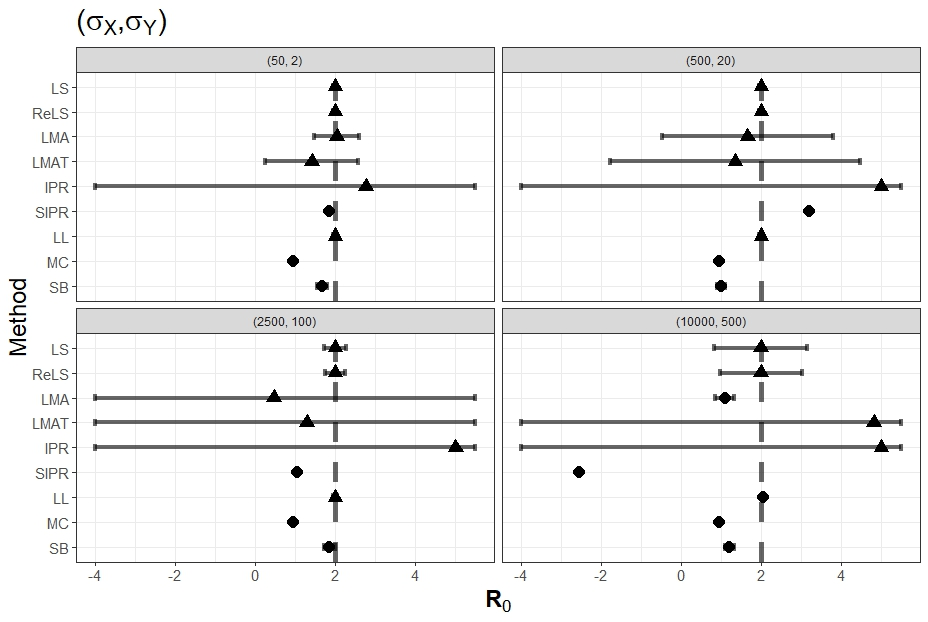
\includegraphics[scale=0.5]{images/var.jpeg}

\begin{table}[H]
	
	\caption{\label{tab:} $(\sigma^2_X, \sigma^2_Y) = (50, 2)$, $\rr$ Estimates and Standard Errors}
	\centering
	\begin{tabular}[t]{l|r|r}
		\hline
		Model & Estimate & Std. Err\\
		\hline
		SIRLS & 1.9997552 & 0.0026502\\
		\hline
		SIRREPAR & 1.9998295 & 0.0023646\\
		\hline
		SIRLMA & 2.0398087 & 0.2773968\\
		\hline
		SIRLMAT & 1.4148628 & 0.5779651\\
		\hline
		SIRIPR & 2.7607518 & 8.1318687\\
		\hline
		SIRSIPR & 1.8368240 & $<$ 1e-07\\
		\hline
		LOGLINEAR & 1.9998907 & 0.0001037\\
		\hline
		SIRMC & 0.9485555 & $<$ 1e-07\\
		\hline
		SEQBAYES & 1.6750053 & 0.0677426\\
		\hline
	\end{tabular}
\end{table}

In the table above, the magnitude of the variance of the noise is smaller than in the baseline. The estimates are closer to the true $/rr$ and the standard errors are smaller across the board. This indicates that the methods give more accurate and precise estimates when the data are closer to following underlying true SIR model.


\begin{table}[H]
	
	\caption{\label{tab:} $(\sigma^2_X, \sigma^2_Y) = (2500, 100)$, $\rr$ Estimates and Standard Errors}
	\centering
	\begin{tabular}[t]{l|r|r}
		\hline
		Model & Estimate & Std. Err\\
		\hline
		SIRLS & 1.9980880 & 0.1353803\\
		\hline
		SIRREPAR & 1.9981446 & 0.1207935\\
		\hline
		SIRLMA & 0.4651913 & 7.5508447\\
		\hline
		SIRLMAT & 1.2877865 & 4.3947658\\
		\hline
		SIRIPR & 81.4901666 & 348.7350849\\
		\hline
		SIRSIPR & 1.0606095 & $<$ 1e-07\\
		\hline
		LOGLINEAR & 2.0018816 & 0.0054085\\
		\hline
		SIRMC & 0.9485562 & 0.0000010\\
		\hline
		SEQBAYES & 1.8567176 & 0.0713225\\
		\hline
	\end{tabular}
\end{table}

In the table above, the magnitude of the variance of the noise is larger than in the baseline. The estimates are worse and the standard errors are larger compared to the baseline data set, which we might expect. These estimates are not as terrible as we might imagine given the magnitude of the change - it seems that these methods are somewhat more robust to large noise compared to other changes. One exception in the IPR model, which may do worse due to larger fluctuations in the incidence prevalence ratio. 

\subsection{Other Models}\label{sec:res-oth}

\begin{table}[H]

  \begin{center}
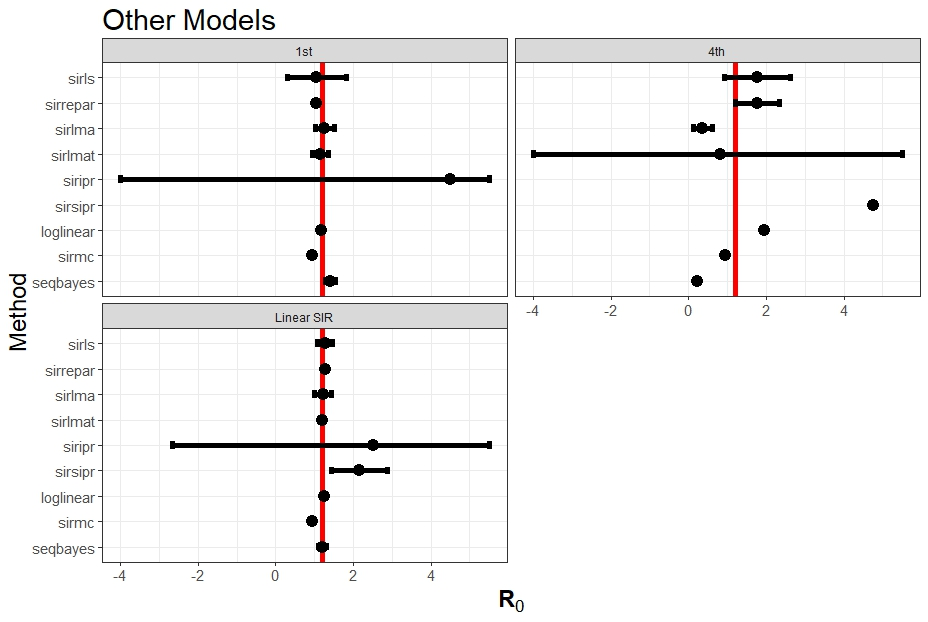
\includegraphics[scale=0.5]{images/other.jpeg}

\end{center}

\caption{\label{tab:} 4th Order Model, $\rr$ Estimates and Standard Errors}
\centering
\begin{tabular}[t]{l|r|r}
	\hline
	Model & Estimate & Std. Dev\\
	\hline
	SIRLS & 1.7693473 & 0.4226615\\
	\hline
	SIRREPAR & 1.7693312 & 0.2796903\\
	\hline
	SIRLMA & 0.3617606 & 0.1231325\\
	\hline
	SIRLMAT & 0.8213066 & 6.0466473\\
	\hline
	SIRIPR & 10.4349388 & 33.8952710\\
	\hline
	SIRSIPR & 4.7477067 &  $<$ 1e-07\\
	\hline
	LOGLINEAR & 1.9551795 & 0.0164608\\
	\hline
	SIRMC & 0.9485545 & 0.0000006\\
	\hline
	SEQBAYES & 0.2118519 & 0.0240918\\
	\hline
\end{tabular}
\end{table}

The table above shows the methods applied to data from a 4th order linear regression model with respect to time. Obviously, there is no true $\rr$ to compare to. What interests us in this case is whether the methods give similar results, since all the estimation methods are derived from the same model. However, the results vary much more compared to baseline data estimates, where underlying data came from SIR. We also get massive standard errors, even though actual noise variance magnitudes are the same as baseline.

\subsection{Repeated Sampling}

\begin{table}[H]
	
	\caption{\label{tab:}Mean $\rr$ Estimates and Std. Devs, Repeated Sampling}
	\centering
	\begin{tabular}[t]{l|r|r|r|r}
		\hline
		Model & Mean Estimate & Std. Dev. & Baseline Estimate & Baseline SE\\
		\hline
		SIRLS & 2.0000175 & 0.0002734 & 1.9999190 & 0.0058322\\
		\hline
		SIRREPAR & 2.0000289 & 0.0003092 & 1.9997083 & 0.0052113\\
		\hline
		SIRLMA & 1.8497054 & 0.3338774 & 1.997416 & 0.3900006\\
		\hline
		SIRLMAT & 1.4562107 & 0.3576736 & 1.398016 & 0.6028170 \\
		\hline
		SIRIPR & 4.5214294 & 0.3705241 & 2.592974 & 9.040841\\
		\hline
		SIRSIPR & 1.7972938 & 0.0951042 & 0.9251762 & $<$ 1e-07 \\
		\hline
		LOGLINEAR & 2.0000079 & 0.0003191 & 1.9998403 & 0.0002227\\
		\hline
		SIRMC & 0.9485555 & $<$ 1e-07 & 0.9485555 & $<$ 1e-07\\
		\hline
		SEQBAYES & 1.1330264 & 0.4163031 & 1.0000000 & 0.0523424\\
		\hline
	\end{tabular}
\end{table}

The table above shows the mean and standard deviation of $/rr$ estimates produced by the models under 100 repetitions of the baseline conditions, with new noise generated each time. We want to compare the standard deviations of the estimates to the standard errors returned by each of the models for a single data set to asses how reliable those standard errors are. Overall, it appears than most of the models have standard error estimates that are smaller than the actual standard deviation of the estimates under repeated sampling. In some cases, such as the log linear method and the linear model approximations, are fairly close. The least squares methods, on the other hand, tend to overestimate the error by an order of magnitude. The SIPR and sequential Bayes model, on the other hand, have individual standard error estimates that are smaller than the standard deviation of repeated estimates, meaning that they understate how much error is in the estimates.

\section{Discussion}\label{sec:discussion}

The SIR estimation methods generally give reliable estimates when the data are from an underlying SIR model with little or no noise. However, the estimates from the various methods are generally much worse when the magnitude of the noise is larger, when the parameters of the model are unusual, and when the model is misspecified. We also see a large difference between the $\rr$ estimates and standard errors on the exact same data sets as well, even though all derived from the same model. Thus, when estimating $/rr$ based on an SIR or any other kind of compartment model, we need to take careful consideration.


\bibliographystyle{apa}%Choose a bibliograhpic style
\bibliography{Master}


\appendix

\section{Beyond the SIR Model}

\section{Fitting the SIR Model}

\subsection{SIR Least Squares}


\begin{table}[H]
	
	\caption{\label{tab:}$\rr$ Estimates and Std. Errs, SIRLS Model,
		$X_0 = 99950, Y_0 = 50$, $\sigma_X = 100, \sigma_Y = 5$, $\beta = 0.06$}
	\centering
	\begin{footnotesize}
		\begin{tabular}[t]{l|r|r|r|r|r|r|r|r}
			\hline
			Data Set & Norm Est & Norm SE & Norm-M Est & Norm-M SE & AR Est & AR SE & AR-M Est & AR-M SE\\
			\hline
			$\gamma$ = 0.001 & 59.9764682 & 0.0434705 & 59.9764682 & 0.0386733 & 60.0151171 & 0.0697888 & 59.9589126 & 0.0631448\\
			\hline
			$\gamma$ = 0.04 & 1.5000763 & 0.0126817 & 1.5001978 & 0.0090880 & 1.4989700 & 0.0182852 & 1.4993603 & 0.0165168\\
			\hline
			$\gamma$ = 0.06 & 1.0043054 & 0.4140424 & 0.9955554 & 0.1086448 & 0.9915431 & 0.6272644 & 0.9941392 & 0.1891812\\
			\hline
			$\gamma$ = 0.24 & 0.2363274 & 4.1042813 & 0.2327691 & 0.6701185 & -0.0695410 & 2.8291362 & 0.3021083 & 0.5657139\\
			\hline
		\end{tabular}
	\end{footnotesize}
\end{table}

\begin{table}[H]
	
	\caption{\label{tab:}$\rr$ Estimates and Std. Errs, SIRLS Model,
		$\sigma_X = 100, \sigma_Y = 5$, $\beta = 0.06, \gamma = 0.03$}
	\centering
	\begin{footnotesize}
		\begin{tabular}[t]{l|r|r|r|r|r|r|r|r}
			\hline
			Data Set & Norm Est & Norm SE & Norm-M Est & Norm-M SE & AR Est & AR SE & AR-M Est & AR-M SE\\
			\hline
			$X_0 = 99000, Y_0 = 1000$ & 1.999588 & 0.0049609 & 2.000284 & 0.0046294 & 2.000461 & 0.0078398 & 2.000122 & 0.0068626\\
			\hline
			$X_0 = 99900, Y_0 = 100$ & 2.022501 & 0.3064263 & 2.021865 & 0.3064148 & 2.022296 & 0.3063477 & 2.022665 & 0.3068512\\
			\hline
			$X_0 = 99990, Y_0 = 10$ & 2.116865 & 0.6626380 & 2.116551 & 0.6621184 & 2.116959 & 0.6623142 & 2.116803 & 0.6620448\\
			\hline
			$X_0 = 99999, Y_0 = 1$ & 2.468304 & 1.5370731 & 2.466776 & 1.5348981 & 2.470607 & 1.5371890 & 2.466700 & 1.5348542\\
			\hline
		\end{tabular}
	\end{footnotesize}
\end{table}

\begin{table}[H]
	\caption{\label{tab:}$\rr$ Estimates and Std. Errs, SIRLS Model,
		$X_0 = 99950, Y_0 = 50$, $\beta = 0.06, \gamma = 0.03$}
	\centering
	\begin{footnotesize}
		\begin{tabular}[t]{l|r|r|r|r|r|r|r|r}
			\hline
			Data Set & Norm Est & Norm SE & Norm-M Est & Norm-M SE & AR Est & AR SE & AR-M Est & AR-M SE\\
			\hline
			$\sigma_X = 50, \sigma_Y = 2$ & 1.999755 & 0.0026502 & 1.999834 & 0.0026397 & 1.999555 & 0.0037664 & 1.999038 & 0.0036473\\
			\hline
			$\sigma_X = 500, \sigma_Y = 20$ & 2.001870 & 0.0259428 & 1.997748 & 0.0162536 & 2.002792 & 0.0416203 & 1.997918 & 0.0257997\\
			\hline
			$\sigma_X = 2500, \sigma_Y = 100$ & 1.998088 & 0.1353803 & 1.996950 & 0.0541332 & 1.999686 & 0.1893888 & 2.002135 & 0.0927952\\
			\hline
			$\sigma_X = 10000, \sigma_Y = 500$ & 1.993455 & 0.5784530 & 1.979966 & 0.1204126 & 2.033934 & 0.7559710 & 2.066706 & 0.3382834\\
			\hline
		\end{tabular}
	\end{footnotesize}
\end{table}

\begin{table}[H]
	
	\caption{\label{tab:}$\rr$ Estimates and Std. Errs, SIRLS Model,
		$X_0 = 99950, Y_0 = 50$, $\sigma_X = 100, \sigma_Y = 5$}
	\centering
	\begin{footnotesize}
		\begin{tabular}[t]{l|r|r|r|r|r|r|r|r}
			\hline
			Data Set & Norm Est & Norm SE & Norm-M Est & Norm-M SE & AR Est & AR SE & AR-M Est & AR-M SE\\
			\hline
			1st Order & 1.051438 & 0.3782910 & 1.051420 & 0.3784628 & 1.051864 & 0.3775363 & 1.051293 & 0.3782570\\
			\hline
			4th Order & 1.769347 & 0.4226615 & 1.769136 & 0.4215768 & 1.769002 & 0.4227615 & 1.769136 & 0.4215910\\
			\hline
			Linear SIR & 1.274258 & 0.0979741 & 1.273917 & 0.0976920 & 1.273654 & 0.1000387 & 1.274007 & 0.0970809\\
			\hline
		\end{tabular}
	\end{footnotesize}
\end{table}

\begin{table}[H]
	
	\caption{\label{tab:}$\rr$ Estimates and Std. Errs, SIRLS Model,
		$\beta = 0.06, \gamma = 0.03$, $X_0 = 99950, Y_0 = 50$, $\sigma_X = 100, \sigma_Y = 5$}
	\centering
	\begin{tabular}[t]{l|r|r|r|r|r|r|r|r}
		\hline
		Data Set & Norm Est & Norm SE & Norm-M Est & Norm-M SE & AR Est & AR SE & AR-M Est & AR-M SE\\
		\hline
		T = 200 & 1.999339 & 0.0286060 & 2.000583 & 0.0204020 & 2.0006557 & 0.0357152 & 2.000722 & 0.0364659\\
		\hline
		T = 100 & 1.990754 & 0.2922125 & 1.993375 & 0.1463550 & 1.9098406 & 0.3811467 & 1.967388 & 0.2324481\\
		\hline
		T = 50 & 1.978167 & 1.1596532 & 1.856227 & 0.3825275 & 2.2720601 & 1.2900031 & 1.699976 & 0.6064311\\
		\hline
		T = 20 & 38.689552 & 106.2705193 & 5.036600 & 1.3672212 & 0.0098756 & 2.1687945 & 1.681588 & 0.4747083\\
		\hline
	\end{tabular}
\end{table}

\subsection{SIR Reparameterization}

\begin{table}[H]
	
	\caption{\label{tab:}$\rr$ Estimates and Std. Errs, SIRREPAR Model,
		$X_0 = 99950, Y_0 = 50$, $\sigma_X = 100, \sigma_Y = 5$, $\beta = 0.06$}
	\centering
	\begin{footnotesize}
		\begin{tabular}[t]{l|r|r|r|r|r|r|r|r}
			\hline
			Data Set & Norm Est & Norm SE & Norm-M Est & Norm-M SE & AR Est & AR SE & AR-M Est & AR-M SE\\
			\hline
			$\gamma$ = 0.001 & 59.995188 & 0.4343984 & 59.9951876 & 0.3874879 & 60.025452 & 0.6911933 & 59.9960910 & 0.6214841\\
			\hline
			$\gamma$ = 0.04 & 1.499883 & 0.0062529 & 1.5001705 & 0.0044936 & 1.499068 & 0.0090313 & 1.4993177 & 0.0081651\\
			\hline
			$\gamma$ = 0.06 & 1.004306 & 0.0501444 & 0.9955446 & 0.0117215 & 0.991558 & 0.0645788 & 0.9941511 & 0.0190525\\
			\hline
			$\gamma$ = 0.24 & 4.179525 & 2.7455569 & 3.5709590 & 0.3171284 & 5.192951 & 3.5249847 & 9.8415034 & 2.5646198\\
			\hline
		\end{tabular}
	\end{footnotesize}
\end{table}

\begin{table}[H]
	
	\caption{\label{tab:}$\rr$ Estimates and Std. Errs, SIRREPAR Model,
		$\sigma_X = 100, \sigma_Y = 5$, $\beta = 0.06, \gamma = 0.03$}
	\centering
	\begin{footnotesize}
		\begin{tabular}[t]{l|r|r|r|r|r|r|r|r}
			\hline
			Data Set & Norm Est & Norm SE & Norm-M Est & Norm-M SE & AR Est & AR SE & AR-M Est & AR-M SE\\
			\hline
			$X_0 = 99000, Y_0 = 1000$ & 1.999712 & 0.0034303 & 2.000274 & 0.0032086 & 2.000082 & 0.0053846 & 2.000014 & 0.0047509\\
			\hline
			$X_0 = 99900, Y_0 = 100$ & 2.022359 & 0.2698034 & 2.021866 & 0.2694871 & 2.022178 & 0.2696002 & 2.022530 & 0.2701860\\
			\hline
			$X_0 = 99990, Y_0 = 10$ & 2.117059 & 0.7291460 & 2.116858 & 0.7290133 & 2.116829 & 0.7288841 & 2.116534 & 0.7286543\\
			\hline
			$X_0 = 99999, Y_0 = 1$  & 2.469189 & 2.7293667 & 2.466967 & 2.7219457 & 2.470707 & 2.7245397 & 2.466483 & 2.7349248\\
			\hline
		\end{tabular}
	\end{footnotesize}
\end{table}

\begin{table}[H]
	
	\caption{\label{tab:}$\rr$ Estimates and Std. Errs, SIRREPAR Model,
		$X_0 = 99950, Y_0 = 50$, $\beta = 0.06, \gamma = 0.03$}
	\centering
	\begin{footnotesize}
		\begin{tabular}[t]{l|r|r|r|r|r|r|r|r}
			\hline
			Data Set & Norm Est & Norm SE & Norm-M Est & Norm-M SE & AR Est & AR SE & AR-M Est & AR-M SE\\
			\hline
			$\sigma_X = 50, \sigma_Y = 2$ & 1.999829 & 0.0023646 & 1.999946 & 0.0023591 & 1.999885 & 0.0033514 & 1.999483 & 0.0032200\\
			\hline
			$\sigma_X = 500, \sigma_Y = 20$ & 2.002305 & 0.0232636 & 1.997996 & 0.0144744 & 2.003065 & 0.0372826 & 1.997732 & 0.0230069\\
			\hline
			$\sigma_X = 2500, \sigma_Y = 100$ & 1.998145 & 0.1207935 & 1.997147 & 0.0481545 & 2.000194 & 0.1680126 & 2.002244 & 0.0826643\\
			\hline
			$\sigma_X = 10000, \sigma_Y = 500$ & 1.993660 & 0.5115266 & 1.979973 & 0.1053955 & 2.033636 & 0.7059701 & 2.066476 & 0.3172823\\
			\hline
		\end{tabular}
	\end{footnotesize}
\end{table}

\begin{table}[H]
	
	\caption{\label{tab:}$\rr$ Estimates and Std. Errs, SIRREPAR Model,
		$X_0 = 99950, Y_0 = 50$, $\sigma_X = 100, \sigma_Y = 5$}
	\centering
	\begin{footnotesize}
		\begin{tabular}[t]{l|r|r|r|r|r|r|r|r}
			\hline
			Data Set & Norm Est & Norm SE & Norm-M Est & Norm-M SE & AR Est & AR SE & AR-M Est & AR-M SE\\
			\hline
			1st Order & 1.051435 & 0.0259416 & 1.051397 & 0.0258690 & 1.051845 & 0.0260146 & 1.051255 & 0.0257166\\
			\hline
			4th Order & 1.769331 & 0.2796903 & 1.769079 & 0.2791191 & 1.769095 & 0.2799270 & 1.769111 & 0.2788789\\
			\hline
			Linear SIR & 1.274314 & 0.0339775 & 1.274075 & 0.0337499 & 1.274174 & 0.0345629 & 1.273799 & 0.0334192\\
			\hline
		\end{tabular}
	\end{footnotesize}
\end{table}

\begin{table}[H]
	
	\caption{\label{tab:}$\rr$ Estimates and Std. Errs, SIRREPAR Model,
		$\beta = 0.06, \gamma = 0.03$, $X_0 = 99950, Y_0 = 50$, $\sigma_X = 100, \sigma_Y = 5$}
	\centering
	\begin{tabular}[t]{l|r|r|r|r|r|r|r|r}
		\hline
		Data Set & Norm Est & Norm SE & Norm-M Est & Norm-M SE & AR Est & AR SE & AR-M Est & AR-M SE\\
		\hline
		T = 200 & 1.999428 & 0.0312814 & 2.000386 & 0.0223765 & 2.000419 & 0.0390441 & 2.000199 & 0.0402489\\
		\hline
		T = 100 & 1.991014 & 0.3940097 & 1.993501 & 0.1974773 & 1.910435 & 0.4773240 & 1.967858 & 0.3065049\\
		\hline
		T = 50 & 1.977508 & 1.8877725 & 1.856480 & 0.5810168 & 2.273215 & 2.3912219 & 1.700025 & 0.7995792\\
		\hline
		T = 20 & 22.964587 & 6.9816713 & 5.044869 & 2.1398099 & NA & NA & 1.681269 & 0.6543603\\
		\hline
	\end{tabular}
\end{table}

\subsection{SIR Linear Model Approximation}

\begin{table}[H]
	
	\caption{\label{tab:}$\rr$ Estimates and Std. Errs, SIRLMA Model,
		$X_0 = 99950, Y_0 = 50$, $\sigma_X = 100, \sigma_Y = 5$, $\beta = 0.06$}
	\centering
	\begin{footnotesize}
		\begin{tabular}[t]{l|r|r|r|r|r|r|r|r}
			\hline
			Data Set & Norm Est & Norm SE & Norm-M Est & Norm-M SE & AR Est & AR SE & AR-M Est & AR-M SE\\
			\hline
			$\gamma$ = 0.001 & -117.9694856 & 101.1885824 & -55.3748542 & 10.9872264 & -19.2057935 & 5.9751126 & -183.9423408 & 277.8291528\\
			\hline
			$\gamma$ = 0.04 & 1.1087585 & 0.0863592 & -3.9728056 & 1116.1887158 & 0.9757401 & 0.0213324 & 0.7333872 & 0.1787735\\
			\hline
			$\gamma$ = 0.06 & 1.0829034 & 0.1533121 & 0.9905684 & 0.1182606 & 0.9279273 & 0.0605799 & 1.0397917 & 0.0359875\\
			\hline
			$\gamma$ = 0.24 & 0.7074613 & 0.2028765 & 0.5216530 & 0.1715628 & 0.8749860 & 0.0590753 & -49.7813412 & 5303.0302298\\
			\hline
		\end{tabular}
	\end{footnotesize}
\end{table}

\begin{table}[H]
	
	\caption{\label{tab:}$\rr$ Estimates and Std. Errs, SIRLMA Model,
		$\sigma_X = 100, \sigma_Y = 5$, $\beta = 0.06, \gamma = 0.03$}
	\centering
	\begin{footnotesize}
		\begin{tabular}[t]{l|r|r|r|r|r|r|r|r}
			\hline
			Data Set & Norm Est & Norm SE & Norm-M Est & Norm-M SE & AR Est & AR SE & AR-M Est & AR-M SE\\
			\hline
			$X_0 = 99000, Y_0 = 1000$ & -87.5945650 & 66413.128046 & -0.9999761 & 1.422640 & 4.1817846 & 3.8812899 & -10.8458320 & 288.1028935\\
			\hline
			$X_0 = 99900, Y_0 = 100$ & 0.5237886 & 1.632971 & 0.2436375 & 3.754091 & 0.7149415 & 0.9374275 & -0.3051038 & 8.8837193\\
			\hline
			$X_0 = 99990, Y_0 = 10$ & -33.0051124 & 433.594227 & -1.3382741 & 3.047220 & -0.2463189 & 1.5875310 & 0.4368556 & 0.7686276\\
			\hline
			$X_0 = 99999, Y_0 = 1$ & 10.9282204 & 19.297359 & -98.6422337 & 3113.332617 & -0.8194023 & 1.7121668 & 16.6102769 & 18.1045393\\
			\hline
		\end{tabular}
	\end{footnotesize}
\end{table}

\begin{table}[H]
	
	\caption{\label{tab:}$\rr$ Estimates and Std. Errs, SIRLMA Model,
		$X_0 = 99950, Y_0 = 50$, $\beta = 0.06, \gamma = 0.03$}
	\centering
	\begin{footnotesize}
		\begin{tabular}[t]{l|r|r|r|r|r|r|r|r}
			\hline
			Data Set & Norm Est & Norm SE & Norm-M Est & Norm-M SE & AR Est & AR SE & AR-M Est & AR-M SE\\
			\hline
			$\sigma_X = 50, \sigma_Y = 2$ & 2.0398087 & 0.2773968 & 1.626788 & 0.0864885 & 1.4643659 & 0.0750183 & 2.8515449 & 0.5540996\\
			\hline
			$\sigma_X = 500, \sigma_Y = 20$ & 1.6600538 & 1.0693161 & 1.684919 & 0.2571470 & 1.1531754 & 0.0997937 & -4.9533560 & 32.2198830\\
			\hline
			$\sigma_X = 2500, \sigma_Y = 100$ & 0.4651914 & 7.5508447 & 4.206167 & 66.2206340 & 1.0391560 & 0.0166472 & -0.1164499 & 1.9126019\\
			\hline
			$\sigma_X = 10000, \sigma_Y = 500$ & 1.0899949 & 0.1202859 & 3.976724 & 4.4279629 & 0.6981674 & 0.2429844 & 1.3944715 & 1.0825033\\
			\hline
		\end{tabular}
	\end{footnotesize}
\end{table}

\begin{table}[H]
	
	\caption{\label{tab:}$\rr$ Estimates and Std. Errs, SIRLMA Model,
		$X_0 = 99950, Y_0 = 50$, $\sigma_X = 100, \sigma_Y = 5$}
	\centering
	\begin{footnotesize}
		\begin{tabular}[t]{l|r|r|r|r|r|r|r|r}
			\hline
			Data Set & Norm Est & Norm SE & Norm-M Est & Norm-M SE & AR Est & AR SE & AR-M Est & AR-M SE\\
			\hline
			1st Order & 1.2559522 & 0.1296269 & 1.2209276 & 0.0597736 & 1.2670255 & 0.1588846 & 1.2476445 & 0.1150267\\
			\hline
			4th Order & 0.3632202 & 0.1230895 & -0.0201429 & 0.1133200 & 0.3580085 & 0.1258904 & -0.0161666 & 0.1103940\\
			\hline
			Linear SIR & 1.2191443 & 0.1093267 & 1.2067608 & 0.0480986 & 1.2146478 & 0.0627181 & 0.9503153 & 0.1066437\\
			\hline
		\end{tabular}
	\end{footnotesize}
\end{table}

\begin{table}[H]
	
	\caption{\label{tab:}$\rr$ Estimates and Std. Errs, SIRLMA Model,
		$\beta = 0.06, \gamma = 0.03$, $X_0 = 99950, Y_0 = 50$, $\sigma_X = 100, \sigma_Y = 5$}
	\centering
	\begin{tabular}[t]{l|r|r|r|r|r|r|r|r}
		\hline
		Data Set & Norm Est & Norm SE & Norm-M Est & Norm-M SE & AR Est & AR SE & AR-M Est & AR-M SE\\
		\hline
		T = 200 & 0.9496498 & 0.0825419 & 1.052892 & 0.2237478 & 1.0611334 & 0.0328849 & 0.7221436 & 0.1920598\\
		\hline
		T = 100 & 1.2374397 & 0.4953607 & 1.202445 & 0.5438859 & 0.9140701 & 0.2563191 & 1.1584230 & 0.3660429\\
		\hline
		T = 50 & 0.9720834 & 0.0507265 & 1.924122 & 1.4342312 & 3.7359315 & 59.4952531 & 0.5305768 & 1.0293919\\
		\hline
		T = 20 & 1.4418031 & 7.3163878 & 1.121779 & 1.7267097 & -5.2984368 & 65.6502768 & 0.8899288 & 0.7605429\\
		\hline
	\end{tabular}
\end{table}

\subsection{SIR Linear Model Approximation, All Time Points}

\begin{table}[H]
	
	\caption{\label{tab:}$\rr$ Estimates and Std. Errs, SIRLMAT Model,
		$X_0 = 99950, Y_0 = 50$, $\sigma_X = 100, \sigma_Y = 5$, $\beta = 0.06$}
	\centering
	\begin{footnotesize}
		\begin{tabular}[t]{l|r|r|r|r|r|r|r|r}
			\hline
			Data Set & Norm Est & Norm SE & Norm-M Est & Norm-M SE & AR Est & AR SE & AR-M Est & AR-M SE\\
			\hline
			$\gamma$ = 0.001 & -2.8535930 & 193.6526107 & 7.7685771 & 103.2205552 & 76.340382 & 472.4155164 & -69.9067922 & 1603.7792325\\
			\hline
			$\gamma$ = 0.04 & 1.4369752 & 0.7498020 & 1.4719115 & 3.0719036 & 1.292978 & 0.3342698 & 1.2769691 & 0.2448445\\
			\hline
			$\gamma$ = 0.06 & 0.9847650 & 0.1423066 & 0.9945574 & 0.0160864 & 1.008112 & 0.5987452 & 1.0268632 & 0.5015724\\
			\hline
			$\gamma$ = 0.24 & 0.6746914 & 6.2471252 & 0.3871567 & 4.8817556 & 1.786500 & 15.9420420 & 0.2221191 & 5.4112205\\
			\hline
		\end{tabular}
	\end{footnotesize}
\end{table}

\begin{table}[H]
	
	\caption{\label{tab:}$\rr$ Estimates and Std. Errs, SIRLMAT Model,
		$\sigma_X = 100, \sigma_Y = 5$, $\beta = 0.06, \gamma = 0.03$}
	\centering
	\begin{footnotesize}
		\begin{tabular}[t]{l|r|r|r|r|r|r|r|r}
			\hline
			Data Set & Norm Est & Norm SE & Norm-M Est & Norm-M SE & AR Est & AR SE & AR-M Est & AR-M SE\\
			\hline
			$X_0 = 99000, Y_0 = 1000$ & 0.730610 & 4.6810416 & 0.9720592 & 0.6586069 & 3.163816 & 45.776770 & 0.9367865 & 0.8857030\\
			\hline
			$X_0 = 99900, Y_0 = 100$ & 1.236415 & 0.7388933 & 1.1744675 & 1.3957615 & 1.249219 & 0.813166 & 1.1960662 & 0.6589163\\
			\hline
			$X_0 = 99990, Y_0 = 10$ & 1.459703 & 10.9219088 & 0.8531016 & 12.5573016 & -3.846910 & 71.297410 & -0.5884883 & 39.4915091\\
			\hline
			$X_0 = 99999, Y_0 = 1$ & 1.624645 & 5.0359845 & 0.4174208 & 12.8380228 & 1.301346 & 25.850056 & 3.1746775 & 12.8142151\\
			\hline
		\end{tabular}
	\end{footnotesize}
\end{table}

\begin{table}[H]
	
	\caption{\label{tab:}$\rr$ Estimates and Std. Errs, SIRLMAT Model,
		$X_0 = 99950, Y_0 = 50$, $\beta = 0.06, \gamma = 0.03$}
	\centering
	\begin{footnotesize}
		\begin{tabular}[t]{l|r|r|r|r|r|r|r|r}
			\hline
			Data Set & Norm Est & Norm SE & Norm-M Est & Norm-M SE & AR Est & AR SE & AR-M Est & AR-M SE\\
			\hline
			$\sigma_X = 50, \sigma_Y = 2$ & 1.414863 & 0.5779651 & 1.509908 & 2.1243768 & 1.3999424 & 0.7193567 & 1.426323 & 0.6782388\\
			\hline
			$\sigma_X = 500, \sigma_Y = 20$ & 1.353711 & 1.5619894 & 1.446169 & 0.7223815 & 1.0183856 & 3.5577619 & 1.996902 & 15.7391571\\
			\hline
			$\sigma_X = 2500, \sigma_Y = 100$ & 1.287786 & 4.3947658 & 1.365338 & 3.2675366 & 1.1984800 & 1.6107382 & 0.942443 & 4.3914050\\
			\hline
			$\sigma_X = 10000, \sigma_Y = 500$ & 4.811335 & 70.6594883 & 1.500486 & 1.0046353 & 0.9241342 & 1.2799734 & 1.097322 & 3.1937985\\
			\hline
		\end{tabular}
	\end{footnotesize}
\end{table}

\begin{table}[H]
	
	\caption{\label{tab:}$\rr$ Estimates and Std. Errs, SIRLMAT Model,
		$X_0 = 99950, Y_0 = 50$, $\sigma_X = 100, \sigma_Y = 5$}
	\centering
	\begin{footnotesize}
		\begin{tabular}[t]{l|r|r|r|r|r|r|r|r}
			\hline
			Data Set & Norm Est & Norm SE & Norm-M Est & Norm-M SE & AR Est & AR SE & AR-M Est & AR-M SE\\
			\hline
			1st Order & 1.1509447 & 0.1012249 & 1.138621 & 0.1738250 & 1.147184 & 0.0681524 & 1.145189 & 0.0811484\\
			\hline
			4th Order & 0.8246203 & 6.0710436 & 1.000597 & 2.5841000 & 3.255953 & 26.3713818 & 1.385674 & 8.5430506\\
			\hline
			Linear SIR & 1.2009801 & 0.0031100 & 1.200130 & 0.0040763 & 1.203159 & 0.0148085 & 1.195875 & 0.0246927\\
			\hline
		\end{tabular}
	\end{footnotesize}
\end{table}

\begin{table}[H]
	
	\caption{\label{tab:}$\rr$ Estimates and Std. Errs, SIRLMAT Model,
		$\beta = 0.06, \gamma = 0.03$, $X_0 = 99950, Y_0 = 50$, $\sigma_X = 100, \sigma_Y = 5$}
	\centering
	\begin{tabular}[t]{l|r|r|r|r|r|r|r|r}
		\hline
		Data Set & Norm Est & Norm SE & Norm-M Est & Norm-M SE & AR Est & AR SE & AR-M Est & AR-M SE\\
		\hline
		T = 200 & 3.3442696 & 21.4895422 & 1.8327212 & 0.2855541 & 1.7170357 & 0.4970127 & 2.294206 & 6.234463\\
		\hline
		T = 100 & 1.2354159 & 3.0461522 & 2.7980661 & 3.8629146 & 0.7524086 & 2.5622573 & 3.434636 & 14.604145\\
		\hline
		T = 50 & 0.7050038 & 2.8719153 & 0.3376738 & 7.9042199 & 0.6897879 & 2.7333396 & 1.274668 & 3.840504\\
		\hline
		T = 20 & 1.0078807 & 0.1424793 & 2.7045722 & 4.8031306 & 0.5716857 & 1.3981528 & 1.449643 & 1.542269\\
		\hline
	\end{tabular}
\end{table}

\subsection{Incidence to Prevalence Ratio}

\begin{table}[H]
	
	\caption{\label{tab:}$\rr$ Estimates and Std. Errs, SIRIPR Model,
		$X_0 = 99950, Y_0 = 50$, $\sigma_X = 100, \sigma_Y = 5$, $\beta = 0.06$}
	\centering
	\begin{footnotesize}
		\begin{tabular}[t]{l|r|r|r|r|r|r|r|r}
			\hline
			Data Set & Norm Est & Norm SE & Norm-M Est & Norm-M SE & AR Est & AR SE & AR-M Est & AR-M SE\\
			\hline
			$\gamma$ = 0.001 & 54.146506 & 200.2595 & 24.408675 & 66.166769 & 58.723744 & 219.989055 & 28.5230747 & 120.928788\\
			\hline
			$\gamma$ = 0.04 & 4.771508 & 12.8533 & 1.387753 & 2.630779 & 3.613754 & 8.536531 & 1.3965600 & 2.840997\\
			\hline
			$\gamma$ = 0.06 & 19.828076 & 29.1272 & 1.121667 & 4.400499 & 15.651052 & 23.539321 & 1.1251847 & 4.900022\\
			\hline
			$\gamma$ = 0.24 & 181.015802 & 742.1088 & 6.672760 & 89.936233 & 148.308767 & 740.018239 & 0.8145271 & 11.870908\\
			\hline
		\end{tabular}
	\end{footnotesize}
\end{table}

\begin{table}[H]
	
	\caption{\label{tab:}$\rr$ Estimates and Std. Errs, SIRIPR Model,
		$\sigma_X = 100, \sigma_Y = 5$, $\beta = 0.06, \gamma = 0.03$}
	\centering
	\begin{footnotesize}
		\begin{tabular}[t]{l|r|r|r|r|r|r|r|r}
			\hline
			Data Set & Norm Est & Norm SE & Norm-M Est & Norm-M SE & AR Est & AR SE & AR-M Est & AR-M SE\\
			\hline
			$X_0 = 99000, Y_0 = 1000$ & 1.285071 & 1.440980 & 0.9866029 & 1.057043 & 1.193594 & 1.195820 & 0.9960353 & 0.9987062\\
			\hline
			$X_0 = 99900, Y_0 = 100$ & 2.943264 & 7.736638 & 1.4707234 & 3.367245 & 2.230244 & 4.859448 & 1.4236604 & 2.8121697\\
			\hline
			$X_0 = 99990, Y_0 = 10$ & 18.663014 & 67.156845 & 1.8455795 & 5.401173 & 16.739763 & 71.982690 & 1.6417916 & 4.4145381\\
			\hline
			$X_0 = 99999, Y_0 = 1$ & 774.274659 & 7491.005080 & 3.6060918 & 26.540940 & 229.184142 & 1199.155653 & 2.5082330 & 12.8639109\\
			\hline
		\end{tabular}
	\end{footnotesize}
\end{table}

\begin{table}[H]
	
	\caption{\label{tab:}$\rr$ Estimates and Std. Errs, SIRIPR Model,
		$X_0 = 99950, Y_0 = 50$, $\beta = 0.06, \gamma = 0.03$}
	\centering
	\begin{footnotesize}
		\begin{tabular}[t]{l|r|r|r|r|r|r|r|r}
			\hline
			Data Set & Norm Est & Norm SE & Norm-M Est & Norm-M SE & AR Est & AR SE & AR-M Est & AR-M SE\\
			\hline
			$\sigma_X = 50, \sigma_Y = 2$ & 1.656451 & 4.879121 & 0.8705396 & 1.231344 & 1.318824 & 3.274114 & 0.8679029 & 1.309243\\
			\hline
			$\sigma_X = 500, \sigma_Y = 20$ & 10.426754 & 42.824909 & 1.1338742 & 4.906623 & 7.750396 & 24.637815 & 1.4241606 & 12.589987\\
			\hline
			$\sigma_X = 2500, \sigma_Y = 100$ & 48.894100 & 209.241051 & 1.3602975 & 10.234817 & 117.222483 & 870.624089 & 1.7544551 & 11.060645\\
			\hline
			$\sigma_X = 10000, \sigma_Y = 500$ & 143.885460 & 778.881724 & 2.7003338 & 35.642540 & 55.265406 & 163.492483 & 2.1210664 & 13.550223\\
			\hline
		\end{tabular}
	\end{footnotesize}
\end{table}

\begin{table}[H]
	
	\caption{\label{tab:}$\rr$ Estimates and Std. Errs, SIRIPR Model,
		$X_0 = 99950, Y_0 = 50$, $\sigma_X = 100, \sigma_Y = 5$}
	\centering
	\begin{footnotesize}
		\begin{tabular}[t]{l|r|r|r|r|r|r|r|r}
			\hline
			Data Set & Norm Est & Norm SE & Norm-M Est & Norm-M SE & AR Est & AR SE & AR-M Est & AR-M SE\\
			\hline
			1st Order & 2.699973 & 9.131131 & 2.297208 & 7.14196 & 4.334767 & 41.325146 & 4.194341 & 36.201142\\
			\hline
			4th Order & 6.260963 & 20.337163 & 5.924029 & 17.81136 & 6.268500 & 20.536192 & 5.892582 & 17.341763\\
			\hline
			Linear SIR & 1.516803 & 1.554241 & 1.208578 & 1.12544 & 1.379871 & 1.311406 & 1.208521 & 1.003065\\
			\hline
		\end{tabular}
	\end{footnotesize}
\end{table}

\begin{table}[H]
	
	\caption{\label{tab:}$\rr$ Estimates and Std. Errs, SIRIPR Model,
		$\beta = 0.06, \gamma = 0.03$, $X_0 = 99950, Y_0 = 50$, $\sigma_X = 100, \sigma_Y = 5$}
	\centering
	\begin{tabular}[t]{l|r|r|r|r|r|r|r|r}
		\hline
		Data Set & Norm Est & Norm SE & Norm-M Est & Norm-M SE & AR Est & AR SE & AR-M Est & AR-M SE\\
		\hline
		T = 200 & 7.345813 & 16.12889 & 2.048281 & 3.959862 & 5.553952 & 13.33904 & 2.052063 & 4.119090\\
		\hline
		T = 100 & 12.683604 & 21.50385 & 2.278429 & 5.329775 & 9.221913 & 18.11852 & 2.245441 & 5.708995\\
		\hline
		T = 50 & 19.220693 & 27.75807 & 2.470106 & 6.581896 & 14.757521 & 24.04262 & 2.616444 & 7.417433\\
		\hline
		T = 20 & 25.731306 & 35.29261 & 1.415537 & 4.565460 & 20.489247 & 33.72596 & 3.885644 & 8.289876\\
		\hline
	\end{tabular}
\end{table}

\subsection{Smoothed Incidence to Prevalence Ratio}


\begin{table}[H]
	
	\caption{\label{tab:}$\rr$ Estimates and Std. Errs, SIRSIPR Model,
		$X_0 = 99950, Y_0 = 50$, $\sigma_X = 100, \sigma_Y = 5$, $\beta = 0.06$}
	\centering
	\begin{footnotesize}
		\begin{tabular}[t]{l|r|r|r|r|r|r|r|r}
			\hline
			Data Set & Norm Est & Norm SE & Norm-M Est & Norm-M SE & AR Est & AR SE & AR-M Est & AR-M SE\\
			\hline
			$\gamma$ = 0.001 & 3.9645187 & $<$ 1e-07 & 3.8285414 & $<$ 1e-07 & 3.9055582 & 0.000000 & 3.7112781 & $<$ 1e-07 \\
			\hline
			$\gamma$ = 0.04 & 1.7451025 & $<$ 1e-07 & 2.8785564 & $<$ 1e-07 & 68.7390000 & 0.000000 & 1.2465750 & $<$ 1e-07 \\
			\hline
			$\gamma$ = 0.06 & 0.9919790 & 0.0559052 & 0.9925620 & 0.0297783 & 0.8718278 & 0.087266 & 1.0294124 & 0.0510585\\
			\hline
			$\gamma$ = 0.24 & -0.2484284 & 0.1159769 & -0.0317365 & 0.0335514 & -2.8642901 & 0.000000 & 0.7365437 & 0.0675331\\
			\hline
		\end{tabular}
	\end{footnotesize}
\end{table}

\begin{table}[H]
	
	\caption{\label{tab:}$\rr$ Estimates and Std. Errs, SIRSIPR Model,
		$\sigma_X = 100, \sigma_Y = 5$, $\beta = 0.06, \gamma = 0.03$}
	\centering
	\begin{footnotesize}
		\begin{tabular}[t]{l|r|r|r|r|r|r|r|r}
			\hline
			Data Set & Norm Est & Norm SE & Norm-M Est & Norm-M SE & AR Est & AR SE & AR-M Est & AR-M SE\\
			\hline
			$X_0 = 99000, Y_0 = 1000$ & 2.0870176 & 57.9229822 & 2.016608 & 57.8153675 & 2.285424 & 57.4382982 & 1.922192 & 57.0457534\\
			\hline
			$X_0 = 99900, Y_0 = 100$ & -0.8808153 & 0.0000000 & -1.150393 & 0.0000000 & -6.563660 & 0.0000000 & -1.777316 & 0.0000000\\
			\hline
			$X_0 = 99990, Y_0 = 10$ & 1.3451986 & 0.3236824 & 1.354925 & 0.3158698 & 1.381198 & 0.3093223 & 1.345069 & 0.3258082\\
			\hline
			$X_0 = 99999, Y_0 = 1$ & 2.4390757 & 0.0000000 & 5.411582 & 0.0000000 & 1.204689 & 0.0000000 & 1.035624 & 0.0000000\\
			\hline
		\end{tabular}
	\end{footnotesize}
\end{table}

\begin{table}[H]
	
	\caption{\label{tab:}$\rr$ Estimates and Std. Errs, SIRSIPR Model,
		$X_0 = 99950, Y_0 = 50$, $\beta = 0.06, \gamma = 0.03$}
	\centering
	\begin{footnotesize}
		\begin{tabular}[t]{l|r|r|r|r|r|r|r|r}
			\hline
			Data Set & Norm Est & Norm SE & Norm-M Est & Norm-M SE & AR Est & AR SE & AR-M Est & AR-M SE\\
			\hline
			$\sigma_X = 50, \sigma_Y = 2$ & 1.836824 & $<$ 1e-07 & 1.7778150 & $<$ 1e-07 & 1.7603970 & $<$ 1e-07 & 1.842289 & $<$ 1e-07 \\
			\hline
			$\sigma_X = 500, \sigma_Y = 20$ & 3.193066 & $<$ 1e-07 & 1.3211468 & $<$ 1e-07 & 1.3509726 & $<$ 1e-07 & 1.334458 & $<$ 1e-07 \\
			\hline
			$\sigma_X = 2500, \sigma_Y = 100$ & 1.060609 & $<$ 1e-07 & 1.2345884 & $<$ 1e-07 & 1.7027546 & $<$ 1e-07 & 2.596160 & $<$ 1e-07 \\
			\hline
			$\sigma_X = 10000, \sigma_Y = 500$ & -2.535946 & $<$ 1e-07 & 0.7094139 & $<$ 1e-07 & 0.8911487 & $<$ 1e-07 & -1.103940 & $<$ 1e-07 \\
			\hline
		\end{tabular}
	\end{footnotesize}
\end{table}

\begin{table}[H]
	
	\caption{\label{tab:}$\rr$ Estimates and Std. Errs, SIRSIPR Model,
		$X_0 = 99950, Y_0 = 50$, $\sigma_X = 100, \sigma_Y = 5$}
	\centering
	\begin{footnotesize}
		\begin{tabular}[t]{l|r|r|r|r|r|r|r|r}
			\hline
			Data Set & Norm Est & Norm SE & Norm-M Est & Norm-M SE & AR Est & AR SE & AR-M Est & AR-M SE\\
			\hline
			1st Order & 58.836635 & $<$ 1e-07 & 27.429685 & $<$ 1e-07 & 1.498805 & $<$ 1e-07 & -14.135196 & $<$ 1e-07 \\
			\hline
			4th Order & 2.848624 & $<$ 1e-07 & 15.083621 & $<$ 1e-07 & 2.766152 & $<$ 1e-07 & 14.972580 & $<$ 1e-07 \\
			\hline
			Linear SIR & 1.294079 & 0.2151131 & 1.294364 & 0.2158095 & 1.296731 & 0.2215603 & 1.304489 & 0.2299876\\
			\hline
		\end{tabular}
	\end{footnotesize}
\end{table}

\begin{table}[H]
	
	\caption{\label{tab:}$\rr$ Estimates and Std. Errs, SIRSIPR Model,
		$\beta = 0.06, \gamma = 0.03$, $X_0 = 99950, Y_0 = 50$, $\sigma_X = 100, \sigma_Y = 5$}
	\centering
	\begin{tabular}[t]{l|r|r|r|r|r|r|r|r}
		\hline
		Data Set & Norm Est & Norm SE & Norm-M Est & Norm-M SE & AR Est & AR SE & AR-M Est & AR-M SE\\
		\hline
		T = 200 & -2.119890 & 0.000000 & 2.6624046 & 0.0000000 & 3.3187716 & 0.0000000 & 2.363125 & 32.2727752\\
		\hline
		T = 100 & 2.341119 & 1.168462 & 2.2020092 & 0.5643447 & 2.0919450 & 1.0699219 & 1.963112 & 0.3489431\\
		\hline
		T = 50 & 2.190565 & 2.238582 & 1.9477092 & 0.4198946 & 1.8701913 & 0.7519526 & 2.279451 & 0.6584392\\
		\hline
		T = 20 & 4.177245 & 7.320297 & 0.9702882 & 0.8673670 & 0.3570221 & 7.6611297 & 3.984916 & 2.1350792\\
		\hline
	\end{tabular}
\end{table}

\subsection{SIR Log Linear}

\begin{table}[H]
	
	\caption{\label{tab:}$\rr$ Estimates and Std. Errs, LOGLINEAR Model,
		$X_0 = 99950, Y_0 = 50$, $\sigma_X = 100, \sigma_Y = 5$, $\beta = 0.06$}
	\centering
	\begin{footnotesize}
		\begin{tabular}[t]{l|r|r|r|r|r|r|r|r}
			\hline
			Data Set & Norm Est & Norm SE & Norm-M Est & Norm-M SE & AR Est & AR SE & AR-M Est & AR-M SE\\
			\hline
			$\gamma$ = 0.001 & 46.3209595 & 0.7797216 & 59.8300371 & 0.1079267 & 41.897714 & 0.9767785 & 70.7075929 & 0.9517239\\
			\hline
			$\gamma$ = 0.04 & 1.5002728 & 0.0001905 & 1.5000436 & 0.0000928 & 1.499516 & 0.0002653 & 1.5000445 & 0.0001481\\
			\hline
			$\gamma$ = 0.06 & 0.9989449 & 0.0007428 & 0.9994831 & 0.0003320 & 1.000275 & 0.0010605 & 1.0008545 & 0.0004910\\
			\hline
			$\gamma$ = 0.24 & 0.9912397 & 0.0030505 & 0.8623034 & 0.0087543 & 1.001367 & 0.0025488 & 0.9198973 & 0.0052616\\
			\hline
		\end{tabular}
	\end{footnotesize}
\end{table}

\begin{table}[H]
	
	\caption{\label{tab:}$\rr$ Estimates and Std. Errs, LOGLINEAR Model,
		$\sigma_X = 100, \sigma_Y = 5$, $\beta = 0.06, \gamma = 0.03$}
	\centering
	\begin{footnotesize}
		\begin{tabular}[t]{l|r|r|r|r|r|r|r|r}
			\hline
			Data Set & Norm Est & Norm SE & Norm-M Est & Norm-M SE & AR Est & AR SE & AR-M Est & AR-M SE\\
			\hline
			$X_0 = 99000, Y_0 = 1000$ & 1.999515 & 0.0002828 & 2.000144 & 0.0001594 & 1.999753 & 0.0004197 & 2.000586 & 0.0003024\\
			\hline
			$X_0 = 99900, Y_0 = 100$ & 2.000011 & 0.0002315 & 1.999732 & 0.0001526 & 2.000473 & 0.0002776 & 2.000640 & 0.0002656\\
			\hline
			$X_0 = 99990, Y_0 = 10$ & 1.999886 & 0.0002517 & 1.999599 & 0.0001361 & 2.000608 & 0.0003289 & 1.999049 & 0.0002664\\
			\hline
			$X_0 = 99999, Y_0 = 1$ & 1.999690 & 0.0007731 & 2.000503 & 0.0003700 & 2.002716 & 0.0010572 & 1.999919 & 0.0005663\\
			\hline
		\end{tabular}
	\end{footnotesize}
\end{table}

\begin{table}[H]
	
	\caption{\label{tab:}$\rr$ Estimates and Std. Errs, LOGLINEAR Model,
		$X_0 = 99950, Y_0 = 50$, $\beta = 0.06, \gamma = 0.03$}
	\centering
	\begin{footnotesize}
		\begin{tabular}[t]{l|r|r|r|r|r|r|r|r}
			\hline
			Data Set & Norm Est & Norm SE & Norm-M Est & Norm-M SE & AR Est & AR SE & AR-M Est & AR-M SE\\
			\hline
			$\sigma_X = 50, \sigma_Y = 2$ & 1.999891 & 0.0001037 & 2.000036 & 0.0000930 & 1.999143 & 0.0001394 & 1.999749 & 0.0001328\\
			\hline
			$\sigma_X = 500, \sigma_Y = 20$ & 2.003402 & 0.0010320 & 1.998765 & 0.0003682 & 2.003763 & 0.0015505 & 1.999829 & 0.0008545\\
			\hline
			$\sigma_X = 2500, \sigma_Y = 100$ & 2.001882 & 0.0054085 & 1.995742 & 0.0015419 & 2.038646 & 0.0081562 & 2.015675 & 0.0031322\\
			\hline
			$\sigma_X = 10000, \sigma_Y = 500$ & 2.059934 & 0.0246402 & 1.995133 & 0.0038894 & 2.209575 & 0.0439100 & 2.545819 & 0.0568537\\
			\hline
		\end{tabular}
	\end{footnotesize}
\end{table}

\begin{table}[H]
	
	\caption{\label{tab:}$\rr$ Estimates and Std. Errs, LOGLINEAR Model,
		$X_0 = 99950, Y_0 = 50$, $\sigma_X = 100, \sigma_Y = 5$}
	\centering
	\begin{footnotesize}
		\begin{tabular}[t]{l|r|r|r|r|r|r|r|r}
			\hline
			Data Set & Norm Est & Norm SE & Norm-M Est & Norm-M SE & AR Est & AR SE & AR-M Est & AR-M SE\\
			\hline
			1st Order & 1.188050 & 0.0006341 & 1.187976 & 0.0006389 & 1.187553 & 0.0006273 & 1.187848 & 0.0006497\\
			\hline
			4th Order & 1.955180 & 0.0164608 & 1.955313 & 0.0164212 & 1.955130 & 0.0164623 & 1.955302 & 0.0164165\\
			\hline
			Linear SIR & 1.258587 & 0.0010079 & 1.258670 & 0.0010069 & 1.258920 & 0.0009938 & 1.258462 & 0.0010199\\
			\hline
		\end{tabular}
	\end{footnotesize}
\end{table}

\begin{table}[H]
	
	\caption{\label{tab:}$\rr$ Estimates and Std. Errs, LOGLINEAR Model,
		$\beta = 0.06, \gamma = 0.03$, $X_0 = 99950, Y_0 = 50$, $\sigma_X = 100, \sigma_Y = 5$}
	\centering
	\begin{tabular}[t]{l|r|r|r|r|r|r|r|r}
		\hline
		Data Set & Norm Est & Norm SE & Norm-M Est & Norm-M SE & AR Est & AR SE & AR-M Est & AR-M SE\\
		\hline
		T = 200 & 2.001415 & 0.0017620 & 2.000649 & 0.0009166 & 2.0053322 & 0.0023026 & 1.992983 & 0.0019266\\
		\hline
		T = 100 & 1.869996 & 0.0322729 & 1.992759 & 0.0104984 & 1.7390224 & 0.0357848 & 2.052393 & 0.0208558\\
		\hline
		T = 50 & 1.193299 & 0.0560189 & 1.741553 & 0.0454525 & 1.2098418 & 0.0420061 & 1.690908 & 0.0406272\\
		\hline
		T = 20 & 1.042976 & 0.0276261 & 1.747193 & 0.3635417 & 0.9170623 & 0.0337569 & 1.432791 & 0.0397426\\
		\hline
	\end{tabular}
\end{table}

\subsection{SIR Markov Chain}

\begin{table}[H]
	
	\caption{\label{tab:}$\rr$ Estimates and Std. Errs, SIRMC Model,
		$X_0 = 99950, Y_0 = 50$, $\sigma_X = 100, \sigma_Y = 5$, $\beta = 0.06$}
	\centering
	\begin{footnotesize}
		\begin{tabular}[t]{l|r|r|r|r|r|r|r|r}
			\hline
			Data Set & Norm Est & Norm SE & Norm-M Est & Norm-M SE & AR Est & AR SE & AR-M Est & AR-M SE\\
			\hline
			$\gamma$ = 0.001 & 0.9485554 & 1.0e-07 & 0.9485555 & $<$ 1e-07 & 0.9485555 & $<$ 1e-07 & 0.9485555 & $<$ 1e-07\\
			\hline
			$\gamma$ = 0.04 & 0.9485555 & $<$ 1e-07 & 0.9485555 & $<$ 1e-07 & 0.9485555 & $<$ 1e-07 & 0.9485555 & $<$ 1e-07\\
			\hline
			$\gamma$ = 0.06 & 0.9485555 & 2.0e-07 & 0.9485555 & $<$ 1e-07 & 0.9485555 & 2.00e-07 & 0.9485555 & $<$ 1e-07\\
			\hline
			$\gamma$ = 0.24 & 0.9485812 & 1.5e-05 & 0.9485605 & 1.4e-06 & 0.9486128 & 1.26e-05 & 0.9485558 & 2e-07\\
			\hline
		\end{tabular}
	\end{footnotesize}
\end{table}

\begin{table}[H]
	
	\caption{\label{tab:}$\rr$ Estimates and Std. Errs, SIRMC Model,
		$\sigma_X = 100, \sigma_Y = 5$, $\beta = 0.06, \gamma = 0.03$}
	\centering
	\begin{footnotesize}
		\begin{tabular}[t]{l|r|r|r|r|r|r|r|r}
			\hline
			Data Set & Norm Est & Norm SE & Norm-M Est & Norm-M SE & AR Est & AR SE & AR-M Est & AR-M SE\\
			\hline
			$X_0 = 99000, Y_0 = 1000$ & 0.9485555 & $<$ 1e-07 & 0.9485555 & $<$ 1e-07 & 0.9485555 & $<$ 1e-07 & 0.9485555 & $<$ 1e-07\\
			\hline
			$X_0 = 99900, Y_0 = 100$ & 0.9485555 & $<$ 1e-07 & 0.9485555 & $<$ 1e-07 & 0.9485555 & $<$ 1e-07 & 0.9485555 & $<$ 1e-07\\
			\hline
			$X_0 = 99990, Y_0 = 10$ & 0.9485552 & 2.00e-07 & 0.9485555 & $<$ 1e-07 & 0.9485558 & 2.0e-07 & 0.9485555 & $<$ 1e-07\\
			\hline
			$X_0 = 99999, Y_0 = 1$ & 0.9486030 & 1.56e-05 & 0.9485557 & $<$ 1e-07 & 0.9485701 & 2.6e-06 & 0.9485555 & $<$ 1e-07\\
			\hline
		\end{tabular}
	\end{footnotesize}
\end{table}

\begin{table}[H]
	
	\caption{\label{tab:}$\rr$ Estimates and Std. Errs, SIRMC Model,
		$X_0 = 99950, Y_0 = 50$, $\beta = 0.06, \gamma = 0.03$}
	\centering
	\begin{footnotesize}
		\begin{tabular}[t]{l|r|r|r|r|r|r|r|r}
			\hline
			Data Set & Norm Est & Norm SE & Norm-M Est & Norm-M SE & AR Est & AR SE & AR-M Est & AR-M SE\\
			\hline
			$\sigma_X = 50, \sigma_Y = 2$ & 0.9485555 & 0.$<$ 1e-07 & 0.9485555 & $<$ 1e-07 & 0.9485555 & 0.$<$ 1e-07 & 0.9485555 & $<$ 1e-07\\
			\hline
			$\sigma_X = 500, \sigma_Y = 20$ & 0.9485554 & 2.0e-07 & 0.9485555 & $<$ 1e-07 & 0.9485554 & 1.0e-07 & 0.9485555 & 1e-07\\
			\hline
			$\sigma_X = 2500, \sigma_Y = 100$ & 0.9485562 & 1.0e-06 & 0.9485554 & 1e-07 & 0.9485640 & 3.6e-06 & 0.9485554 & 1e-07\\
			\hline
			$\sigma_X = 10000, \sigma_Y = 500$ & 0.9485506 & 3.8e-06 & 0.9485556 & 2e-07 & 0.9485428 & 2.6e-06 & 0.9485538 & 8e-07\\
			\hline
		\end{tabular}
	\end{footnotesize}
\end{table}

\begin{table}[H]
	
	\caption{\label{tab:}$\rr$ Estimates and Std. Errs, SIRMC Model,
		$X_0 = 99950, Y_0 = 50$, $\sigma_X = 100, \sigma_Y = 5$}
	\centering
	\begin{footnotesize}
		\begin{tabular}[t]{l|r|r|r|r|r|r|r|r}
			\hline
			Data Set & Norm Est & Norm SE & Norm-M Est & Norm-M SE & AR Est & AR SE & AR-M Est & AR-M SE\\
			\hline
			1st Order & 0.9485551 & 1e-07 & 0.9485540 & 4e-07 & 0.9485555 & 2e-07 & 0.9485553 & 2.0e-07\\
			\hline
			4th Order & 0.9485545 & 6e-07 & 0.9485533 & 1e-06 & 0.9485535 & 9e-07 & 0.9485527 & 1.2e-06\\
			\hline
			Linear SIR & 0.9485555 & $<$ 1e-07 & 0.9485555 & $<$ 1e-07 & 0.9485555 & $<$ 1e-07 & 0.9485555 & 0.$<$ 1e-07\\
			\hline
		\end{tabular}
	\end{footnotesize}
\end{table}

\begin{table}[H]
	
	\caption{\label{tab:}$\rr$ Estimates and Std. Errs, SIRMC Model,
		$\beta = 0.06, \gamma = 0.03$, $X_0 = 99950, Y_0 = 50$, $\sigma_X = 100, \sigma_Y = 5$}
	\centering
	\begin{tabular}[t]{l|r|r|r|r|r|r|r|r}
		\hline
		Data Set & Norm Est & Norm SE & Norm-M Est & Norm-M SE & AR Est & AR SE & AR-M Est & AR-M SE\\
		\hline
		T = 200 & 0.9485555 & 1e-07 & 0.9485555 & $<$ 1e-07 & 0.9485555 & $<$ 1e-07 & 0.9485555 & $<$ 1e-07\\
		\hline
		T = 100 & 0.9485555 & 1e-07 & 0.9485555 & $<$ 1e-07 & 0.9485555 & 1e-07 & 0.9485555 & $<$ 1e-07\\
		\hline
		T = 50 & 0.9485554 & 2e-07 & 0.9485555 & $<$ 1e-07 & 0.9485555 & 2e-07 & 0.9485555 & $<$ 1e-07\\
		\hline
		T = 20 & 0.9485556 & 5e-07 & 0.9485554 & $<$ 1e-07 & 0.9485552 & 5e-07 & 0.9485556 & 1e-07\\
		\hline
	\end{tabular}
\end{table}

\subsection{SIR Sequential Bayes}

\begin{table}[H]
	
	\caption{\label{tab:}$\rr$ Estimates and Std. Errs, SEQBAYES Model,
		$X_0 = 99950, Y_0 = 50$, $\sigma_X = 100, \sigma_Y = 5$, $\beta = 0.06$}
	\centering
	\begin{footnotesize}
	\begin{tabular}[t]{l|r|r|r|r|r|r|r|r}
		\hline
		Data Set & Norm Est & Norm SE & Norm-M Est & Norm-M SE & AR Est & AR SE & AR-M Est & AR-M SE\\
		\hline
		$\gamma$ = 0.001 & 0.9769731 & 0.0517362 & 1.000000 & 0.0523424 & 1.000000 & 0.0523424 & 1.000000 & 0.0523424\\
		\hline
		$\gamma$ = 0.04 & 1.2060946 & 0.0574836 & 1.000000 & 0.0523424 & 1.073894 & 0.0542418 & 1.115316 & 0.0552780\\
		\hline
		$\gamma$ = 0.06 & 1.0000000 & 0.0523424 & 1.000000 & 0.0523424 & 0.640393 & 0.0418868 & 1.000000 & 0.0523424\\
		\hline
		$\gamma$ = 0.24 & 1.2354952 & 0.0581800 & 1.338591 & 0.0605588 & 1.009694 & 0.0525955 & 1.000000 & 0.0523424\\
		\hline
	\end{tabular}
\end{footnotesize}
\end{table}


\begin{table}[H]
	
	\caption{\label{tab:}$\rr$ Estimates and Std. Errs, SEQBAYES Model,
		$\sigma_X = 100, \sigma_Y = 5$, $\beta = 0.06, \gamma = 0.03$}
	\centering
	\begin{footnotesize}
		\begin{tabular}[t]{l|r|r|r|r|r|r|r|r}
			\hline
			Data Set & Norm Est & Norm SE & Norm-M Est & Norm-M SE & AR Est & AR SE & AR-M Est & AR-M SE\\
			\hline
			$X_0 = 99000, Y_0 = 1000$ & 0.9728534 & 0.0516270 & 1.052579 & 0.0537008 & 0.5850802 & 0.0400370 & 0.6236582 & 0.0413358\\
			\hline
			$X_0 = 99900, Y_0 = 100$ & 1.0000000 & 0.0523424 & 1.000000 & 0.0523424 & 1.4175193 & 0.0623186 & 1.4017333 & 0.0619707\\
			\hline
			$X_0 = 99990, Y_0 = 10$ & 1.3877095 & 0.0616599 & 1.430888 & 0.0626118 & 1.3948200 & 0.0618177 & 1.4507203 & 0.0630442\\
			\hline
			$X_0 = 99999, Y_0 = 1$ & 1.4714813 & 0.0634938 & 1.465728 & 0.0633695 & 1.4665442 & 0.0633871 & 1.4723265 & 0.0635120\\
			\hline
		\end{tabular}
	\end{footnotesize}
\end{table}

\begin{table}[H]
	
	\caption{\label{tab:}$\rr$ Estimates and Std. Errs, SEQBAYES Model,
		$X_0 = 99950, Y_0 = 50$, $\beta = 0.06, \gamma = 0.03$}
	\centering
	\begin{footnotesize}
	\begin{tabular}[t]{l|r|r|r|r|r|r|r|r}
		\hline
		Data Set & Norm Est & Norm SE & Norm-M Est & Norm-M SE & AR Est & AR SE & AR-M Est & AR-M SE\\
		\hline
		$\sigma_X = 50, \sigma_Y = 2$ & 1.409094 & 0.0621332 & 1.141402 & 0.0559207 & 1.386553 & 0.0616342 & 1.336668 & 0.0605153\\
		\hline
		$\sigma_X = 500, \sigma_Y = 20$ & 1.000000 & 0.0523424 & 1.415487 & 0.0622740 & 1.000000 & 0.0523424 & 1.000000 & 0.0523424\\
		\hline
		$\sigma_X = 2500, \sigma_Y = 100$ & 1.519223 & 0.0645155 & 1.000000 & 0.0523424 & 1.549862 & 0.0651629 & 1.000000 & 0.0523424\\
		\hline
		$\sigma_X = 10000, \sigma_Y = 500$ & 1.127679 & 0.0555836 & 1.000000 & 0.0523424 & 1.540929 & 0.0649748 & 1.000000 & 0.0523424\\
		\hline
	\end{tabular}
\end{footnotesize}
\end{table}

\begin{table}[H]
	
	\caption{\label{tab:}$\rr$ Estimates and Std. Errs, SEQBAYES Model,
		$X_0 = 99950, Y_0 = 50$, $\sigma_X = 100, \sigma_Y = 5$}
	\centering
	\begin{footnotesize}
	\begin{tabular}[t]{l|r|r|r|r|r|r|r|r}
		\hline
		Data Set & Norm Est & Norm SE & Norm-M Est & Norm-M SE & AR Est & AR SE & AR-M Est & AR-M SE\\
		\hline
		1st Order & 1.2515351 & 0.0585565 & 1.221050 & 0.0578389 & 1.301757 & 0.0597198 & 1.2848494 & 0.0593307\\
		\hline
		4th Order & 0.5223345 & 0.0378293 & 0.550362 & 0.0388309 & 0.523122 & 0.0378578 & 0.5506554 & 0.0388413\\
		\hline
		Linear SIR & 1.1217433 & 0.0554371 & 1.194507 & 0.0572068 & 1.123600 & 0.0554829 & 1.1568274 & 0.0562973\\
		\hline
	\end{tabular}
	\end{footnotesize}
\end{table}

\begin{table}[H]
	
	\caption{\label{tab:}$\rr$ Estimates and Std. Errs, SEQBAYES Model,
		$\beta = 0.06, \gamma = 0.03$, $X_0 = 99950, Y_0 = 50$, $\sigma_X = 100, \sigma_Y = 5$}
	\centering
	\begin{tabular}[t]{l|r|r|r|r|r|r|r|r}
		\hline
		Data Set & Norm Est & Norm SE & Norm-M Est & Norm-M SE & AR Est & AR SE & AR-M Est & AR-M SE\\
		\hline
		T = 200 & 1.675005 & 0.0677426 & 1.233313 & 0.0581286 & 1.637813 & 0.0669862 & 1.555502 & 0.0652813\\
		\hline
		T = 100 & 1.000000 & 0.0523424 & 1.685553 & 0.0679555 & 1.000000 & 0.0523424 & 1.000000 & 0.0523424\\
		\hline
		T = 50 & 1.856718 & 0.0713225 & 1.000000 & 0.0523424 & 1.907273 & 0.0722870 & 1.000000 & 0.0523424\\
		\hline
		T = 20 & 1.210671 & 0.0575926 & 1.000000 & 0.0523424 & 1.892533 & 0.0720071 & 1.000000 & 0.0523424\\
		\hline
	\end{tabular}
\end{table}

\subsection{Exponential Growth}

\begin{table}[H]
	
	\caption{\label{tab:}$\rr$ Estimates and Std. Errs, EXPGROWTH Model,
		$\beta = 0.06, \gamma = 0.03$, $X_0 = 99950, Y_0 = 50$, $\sigma_X = 100, \sigma_Y = 5$}
	\centering
	\begin{tabular}[t]{l|r|r|r|r|r|r|r|r}
		\hline
		Data Set & Norm Est & Norm SE & Norm-M Est & Norm-M SE & AR Est & AR SE & AR-M Est & AR-M SE\\
		\hline
		$\gamma$ = 0.001 & 1.141015 & 0.0001503 & 1.1349235 & 0.0001645 & 1.139834 & 0.0001529 & 1.1348807 & 0.0001646\\
		\hline
		$\gamma$ = 0.04 & 1.133308 & 0.0001686 & 1.1310087 & 0.0001744 & 1.132539 & 0.0001705 & 1.1313483 & 0.0001735\\
		\hline
		$\gamma$ = 0.06 & 1.093381 & 0.0003053 & 0.9905347 & 0.0013816 & 1.085491 & 0.0003433 & 0.9899559 & 0.0013931\\
		\hline
		$\gamma$ = 0.24 & 1.092493 & 0.0003093 & 0.9206087 & 0.0036121 & 1.085583 & 0.0003428 & 0.8860333 & 0.0055673\\
		\hline
	\end{tabular}
\end{table}

\begin{table}[H]
	
	\caption{\label{tab:}$\rr$ Estimates and Std. Errs, EXPGROWTH Model,
		$\beta = 0.06, \gamma = 0.03$, $X_0 = 99950, Y_0 = 50$, $\sigma_X = 100, \sigma_Y = 5$}
	\centering
	\begin{tabular}[t]{l|r|r|r|r|r|r|r|r}
		\hline
		Data Set & Norm Est & Norm SE & Norm-M Est & Norm-M SE & AR Est & AR SE & AR-M Est & AR-M SE\\
		\hline
		$X_0 = 99000, Y_0 = 1000$ & 1.132250 & 0.0001712 & 1.127900 & 0.0001827 & 1.131379 & 0.0001734 & 1.127954 & 0.0001825\\
		\hline
		$X_0 = 99900, Y_0 = 100$ & 1.143191 & 0.0001455 & 1.141440 & 0.0001494 & 1.142493 & 0.0001470 & 1.141621 & 0.0001489\\
		\hline
		$X_0 = 99990, Y_0 = 10$ & 1.148203 & 0.0001351 & 1.147130 & 0.0001372 & 1.148093 & 0.0001353 & 1.147197 & 0.0001371\\
		\hline
		$X_0 = 99999, Y_0 = 1$& 1.140076 & 0.0001524 & 1.136283 & 0.0001612 & 1.138602 & 0.0001558 & 1.136402 & 0.0001610\\
		\hline
	\end{tabular}
\end{table}

\begin{table}[H]
	
	\caption{\label{tab:}$\rr$ Estimates and Std. Errs, EXPGROWTH Model,
		$\beta = 0.06, \gamma = 0.03$, $X_0 = 99950, Y_0 = 50$}
	\centering
	\begin{tabular}[t]{l|r|r|r|r|r|r|r|r}
		\hline
		Data Set & Norm Est & Norm SE & Norm-M Est & Norm-M SE & AR Est & AR SE & AR-M Est & AR-M SE\\
		\hline
		$\sigma_X = 50, \sigma_Y = 2$ & 1.144401 & 0.0001429 & 1.144116 & 0.0001435 & 1.144199 & 0.0001433 & 1.144083 & 0.0001436\\
		\hline
		$\sigma_X = 500, \sigma_Y = 20$ & 1.161010 & 0.0001117 & 1.144155 & 0.0001434 & 1.157193 & 0.0001182 & 1.143996 & 0.0001438\\
		\hline
		$\sigma_X = 2500, \sigma_Y = 100$ & 1.203070 & 0.0000599 & 1.144496 & 0.0001427 & 1.195816 & 0.0000667 & 1.147499 & 0.0001365\\
		\hline
		$\sigma_X = 10000, \sigma_Y = 500$ & 1.248181 & 0.0000309 & 1.146211 & 0.0001391 & 1.237044 & 0.0000364 & 1.156277 & 0.0001198\\
		\hline
	\end{tabular}
\end{table}

\begin{table}[H]
	
	\caption{\label{tab:}$\rr$ Estimates and Std. Errs, EXPGROWTH Model,
		$X_0 = 99950, Y_0 = 50$, $\sigma_X = 100, \sigma_Y = 5$}
	\centering
	\begin{tabular}[t]{l|r|r|r|r|r|r|r|r}
		\hline
		Data Set & Norm Est & Norm SE & Norm-M Est & Norm-M SE & AR Est & AR SE & AR-M Est & AR-M SE\\
		\hline
		1st Order & 1.061431 & 0.0004905 & 1.060632 & 0.0004964 & 1.060995 & 0.0004937 & 1.061004 & 0.0004936\\
		\hline
		4th Order & 1.148524 & 0.0001344 & 1.148405 & 0.0001347 & 1.148513 & 0.0001344 & 1.148399 & 0.0001347\\
		\hline
		Linear SIR & 1.087741 & 0.0003320 & 1.087338 & 0.0003340 & 1.087538 & 0.0003330 & 1.087399 & 0.0003337\\
		\hline
	\end{tabular}
\end{table}

\begin{table}[H]
	
	\caption{\label{tab:}$\rr$ Estimates and Std. Errs, EXPGROWTH Model,
		$\beta = 0.06, \gamma = 0.03$, $X_0 = 99950, Y_0 = 50$, $\sigma_X = 100, \sigma_Y = 5$}
	\centering
	\begin{tabular}[t]{l|r|r|r|r|r|r|r|r}
		\hline
		Data Set & Norm Est & Norm SE & Norm-M Est & Norm-M SE & AR Est & AR SE & AR-M Est & AR-M SE\\
		\hline
		T = 200 & 1.306607 & 0.0004142 & 1.301989 & 0.0004286 & 1.304421 & 0.0004209 & 1.301390 & 0.0004305\\
		\hline
		T = 100 & 1.560029 & 0.0022192 & 1.418887 & 0.0035072 & 1.517223 & 0.0025481 & 1.390702 & 0.0038451\\
		\hline
		T = 50 & 2.238028 & 0.0078639 & 1.623615 & 0.0184718 & 2.186315 & 0.0084553 & 1.634726 & 0.0181912\\
		\hline
		T = 20 & 4.472654 & 0.0339963 & 1.108447 & 0.1728373 & 4.159546 & 0.0412621 & 2.711197 & 0.0923793\\
		\hline
	\end{tabular}
\end{table}

\subsection{Wallinga}

\begin{table}[H]
	
	\caption{\label{tab:}$\rr$ Estimates and Std. Errs, WALLINGA Model,
		$\beta = 0.06, \gamma = 0.03$, $X_0 = 99950, Y_0 = 50$, $\sigma_X = 100, \sigma_Y = 5$}
	\centering
	\begin{tabular}[t]{l|r|r|r|r|r|r|r|r}
		\hline
		Data Set & Norm Est & Norm SE & Norm-M Est & Norm-M SE & AR Est & AR SE & AR-M Est & AR-M SE\\
		\hline
		$\gamma$ = 0.001 & 1.114829 & 0.0459625 & 0.9591728 & 0.0488597 & 1.140804 & 0.0459639 & 0.8574921 & 0.0500578\\
		\hline
		$\gamma$ = 0.04 & 2.008614 & 0.0318940 & 2.0086026 & 0.0318958 & 2.008640 & 0.0318947 & 2.0086160 & 0.0318934\\
		\hline
		$\gamma$ = 0.06 & 2.038747 & 0.0313772 & 2.0387516 & 0.0313766 & 2.038764 & 0.0313758 & 2.0387101 & 0.0313764\\
		\hline
		$\gamma$ = 0.24 & 2.039700 & 0.0313775 & 2.0397001 & 0.0313775 & 2.039712 & 0.0313791 & 2.0396914 & 0.0313784\\
		\hline
	\end{tabular}
\end{table}

\begin{table}[H]
	
	\caption{\label{tab:}$\rr$ Estimates and Std. Errs, WALLINGA Model,
		$\beta = 0.06, \gamma = 0.03$, $X_0 = 99950, Y_0 = 50$, $\sigma_X = 100, \sigma_Y = 5$}
	\centering
	\begin{tabular}[t]{l|r|r|r|r|r|r|r|r}
		\hline
		Data Set & Norm Est & Norm SE & Norm-M Est & Norm-M SE & AR Est & AR SE & AR-M Est & AR-M SE\\
		\hline
		$X_0 = 99000, Y_0 = 1000$ & 1.873533 & 0.0318531 & 1.873446 & 0.0318541 & 1.873475 & 0.0318524 & 1.873496 & 0.0318549\\
		\hline
		$X_0 = 99900, Y_0 = 100$ & 1.923607 & 0.0328651 & 1.923653 & 0.0328648 & 1.923560 & 0.0328664 & 1.923576 & 0.0328694\\
		\hline
		$X_0 = 99990, Y_0 = 10$ & 1.979338 & 0.0325801 & 1.979345 & 0.0325796 & 1.979353 & 0.0325789 & 1.979404 & 0.0325774\\
		\hline
		$X_0 = 99999, Y_0 = 1$& 2.022337 & 0.0317890 & 2.022325 & 0.0317883 & 2.022367 & 0.0317860 & 2.022322 & 0.0317898\\
		\hline
	\end{tabular}
\end{table}

\begin{table}[H]
	
	\caption{\label{tab:}$\rr$ Estimates and Std. Errs, WALLINGA Model,
		$\beta = 0.06, \gamma = 0.03$, $X_0 = 99950, Y_0 = 50$}
	\centering
	\begin{tabular}[t]{l|r|r|r|r|r|r|r|r}
		\hline
		Data Set & Norm Est & Norm SE & Norm-M Est & Norm-M SE & AR Est & AR SE & AR-M Est & AR-M SE\\
		\hline
		$\sigma_X = 50, \sigma_Y = 2$ & 1.940295 & 0.0328946 & 1.940280 & 0.0328946 & 1.940313 & 0.0328958 & 1.940303 & 0.0328948\\
		\hline
		$\sigma_X = 500, \sigma_Y = 20$ & 1.940066 & 0.0328982 & 1.940463 & 0.0328877 & 1.939755 & 0.0329040 & 1.940506 & 0.0328904\\
		\hline
		$\sigma_X = 2500, \sigma_Y = 100$ & 1.940497 & 0.0328856 & 1.940101 & 0.0329012 & 1.937796 & 0.0329248 & 1.938458 & 0.0329298\\
		\hline
		$\sigma_X = 10000, \sigma_Y = 500$ & 1.934924 & 0.0329764 & 1.942861 & 0.0328652 & 1.910502 & 0.0346809 & 1.913664 & 0.0339201\\
		\hline
	\end{tabular}
\end{table}

\begin{table}[H]
	
	\caption{\label{tab:}$\rr$ Estimates and Std. Errs, WALLINGA Model,
		$X_0 = 99950, Y_0 = 50$, $\sigma_X = 100, \sigma_Y = 5$}
	\centering
	\begin{tabular}[t]{l|r|r|r|r|r|r|r|r}
		\hline
		Data Set & Norm Est & Norm SE & Norm-M Est & Norm-M SE & AR Est & AR SE & AR-M Est & AR-M SE\\
		\hline
		1st Order & 2.034020 & 0.0314227 & 2.034020 & 0.0314227 & 2.034018 & 0.0314231 & 2.034013 & 0.0314227\\
		\hline
		4th Order & 1.938669 & 0.0331254 & 1.938646 & 0.0331271 & 1.938678 & 0.0331252 & 1.938644 & 0.0331271\\
		\hline
		Linear SIR & 2.033555 & 0.0314612 & 2.033554 & 0.0314611 & 2.033555 & 0.0314609 & 2.033547 & 0.0314615\\
		\hline
	\end{tabular}
\end{table}

\begin{table}[H]
	
	\caption{\label{tab:}$\rr$ Estimates and Std. Errs, WALLINGA Model,
		$\beta = 0.06, \gamma = 0.03$, $X_0 = 99950, Y_0 = 50$, $\sigma_X = 100, \sigma_Y = 5$}
	\centering
	\begin{tabular}[t]{l|r|r|r|r|r|r|r|r}
		\hline
		Data Set & Norm Est & Norm SE & Norm-M Est & Norm-M SE & AR Est & AR SE & AR-M Est & AR-M SE\\
		\hline
		T = 200 & 2.872029 & 0.0777506 & 2.872039 & 0.0777500 & 2.872024 & 0.0777475 & 2.871995 & 0.0777522\\
		\hline
		T = 100 & 4.777225 & 0.2173201 & 4.777183 & 0.2173166 & 4.777046 & 0.2173274 & 4.777196 & 0.2173002\\
		\hline
		T = 50 & 8.523307 & 0.6084195 & 8.523224 & 0.6084023 & 8.523328 & 0.6084437 & 8.523118 & 0.6083556\\
		\hline
		T = 20 & 19.536946 & 2.3356802 & 19.536830 & 2.3354926 & 19.537515 & 2.3353411 & 19.534388 & 2.3356299\\
		\hline
	\end{tabular}
\end{table}

\end{document}


%%%%%%%%%%%%%%%%%%%%%%
\textbf{Title:} 

\textbf{Author:} 

\textbf{Citation:} 

\textbf{Major themes:} 

\textbf{Notes:}
\\
%%%%%%%%%%%%%%%%%%%%%%




\begin{figure}[h]
\begin{center}
\includegraphics[width=4in]{images/mvhw7_3c.pdf}
\end{center}
\caption{
Biplots of the different continuous variables and their correlations.}\label{fig3c}
\end{figure}

%% two pictures whoa

\begin{figure}[h]
\centering


\begin{figure}[h]
\centering

\begin{subfigure}{.5\textwidth}
  \centering
  \includegraphics[width=1\linewidth]{images/mt_eda_cont_hists.pdf}
  \caption{Histograms of Arrival Delay and continuous covariates.  Arrival delay seems to have a right skewed distribution.  This may indicate that we will be transforming this variable later on.  After transforming Air Time and Distance by a log transformation, we don't really seem to have many outliers in our covariates.  We seem to have outliers in the CRS Dep. Time and Arrival Time; however, time is cyclical and so these are not, in fact outliers.}
  \label{hists}
\end{subfigure}%
\begin{subfigure}{.5\textwidth}
  \centering
  \includegraphics[width=1\linewidth]{images/mt_eda_cont_hists.pdf}
  \caption{\textcolor{red}{Placeholder}}
  \label{tabs1}
\end{subfigure}
\caption{}
\end{figure}


\begin{table}
\begin{tabular}{l | a | b | a | b}
\hline
\rowcolor{LightCyan}
\mc{1}{}  & \mc{1}{x} & \mc{1}{y} & \mc{1}{w} & \mc{1}{z} \    \hline
variable 1 & a & b & c & d \    variable 2 & a & b & c & d \\ \hline
\end{tabular}
\end{table}






%%
\begin{figure}
\centering
\begin{subfigure}{.5\textwidth}
  \centering
  \includegraphics[width=1\linewidth]{images/resids_full.pdf}
  \caption{}
  \label{residsf}
\end{subfigure}%
\begin{subfigure}{.5\textwidth}
  \centering
  \includegraphics[width=1\linewidth]{images/diags_full.pdf}
  \caption{ }
  \label{diagsf}
\end{subfigure}
\caption{}
\end{figure}





\message{ !name(draft_v13.tex) !offset(-2294) }
